\documentclass{article}
\usepackage{graphicx} % Required for inserting images
\usepackage{amsmath}
\usepackage{url}  
\usepackage[sorting=none,backend=biber]{biblatex}
\addbibresource{sample.bib}
\title{Computational Methods for Material Science}

\author{ALESSANDRO CROTTI}
\date{May 2025}

\begin{document}

\maketitle


\section{Introduction}

Crystalline silicon (Si) is the cornerstone of the modern semiconductor industry, and its technological dominance is rooted in its unique structural, electronic, and vibrational properties. A deep understanding of these fundamental characteristics at the atomic scale is essential for the continued advancement of electronic and photonic devices. Computational modeling, particularly Density Functional Theory (DFT), has become an indispensable tool for achieving this understanding, offering predictive power that complements and often guides experimental research.

This work presents a comprehensive computational study of bulk silicon using the Quantum ESPRESSO software suite. Our objective is to systematically characterize its fundamental properties through first-principles calculations and to rigorously validate our findings against established experimental data. We pursue a multi-faceted approach:
\begin{enumerate}
    \item We first establish the structural ground state by determining the equilibrium lattice constant and bulk modulus via an equation of state analysis, preceded by a careful study of computational convergence.
    \item We then explore the electronic properties by calculating the band structure and the Density of States (DOS), with a focus on identifying the nature and magnitude of the electronic band gap.
    \item Finally, we probe the lattice dynamics by computing the frequency of the zone-center optical phonon using an \textit{ab initio} molecular dynamics approach.
\end{enumerate}

Throughout this study, our calculated results are compared with established experimental values, not only to validate our methodology but also to highlight the predictive power and the inherent limitations of the PBE exchange-correlation functional for describing semiconductor materials.




\section{Computational Methodology}

All calculations presented in this work were performed within the framework of Density Functional Theory (DFT) \cite{hohenberg_kohn_1964, kohn_sham_1965}, as implemented in the Quantum ESPRESSO software suite \cite{qe_2009, qe_2017}. For the exchange-correlation energy, we employed the Generalized Gradient Approximation (GGA) with the Perdew-Burke-Ernzerhof (PBE) functional \cite{pbe_1996}. The interaction between the ionic cores and the valence electrons was described using norm-conserving pseudopotentials.

Our system of study is crystalline silicon (Si) in the diamond cubic structure. In Quantum ESPRESSO, this corresponds to the face-centered cubic (FCC) Bravais lattice with a two-atom basis, specified by the \verb|ibrav=2| and \verb|nat=2| parameters. The crystal structure is defined by a single lattice parameter, \verb|celldm(1)| = $a$, which represents the side length of the conventional cubic cell. The volume of the primitive cell, containing two atoms, is therefore given by $V_{cell} = a^3/4$. This relation is used to calculate the volume for the equation of state analysis.

\section{Equilibrium Lattice Constant and Bulk Modulus}

The first step in any DFT study is to determine the optimal computational parameters that guarantee numerically converged results. These parameters, primarily the plane-wave kinetic energy cutoff (\verb|ecutwfc|) and the density of the k-point mesh for Brillouin zone integration, must be chosen such that the calculated total energy is independent of their value.

\subsection{Convergence Study}

To find the optimal parameters, we performed a two-step convergence analysis.
First, we determined the required energy cutoff. Keeping the k-point mesh fixed at a reasonably dense \verb|6x6x6| grid and the lattice parameter at $a=10.2$ Bohr, we performed a series of self-consistent field (SCF) calculations, varying `ecutwfc` from $20$ Ry to $60$ Ry. As shown in Figure \ref{fig:en-ecut}, the total energy progressively decreases and stabilizes as the cutoff increases. To establish a precise convergence threshold, we analyzed the energy difference between successive steps (Figure \ref{fig:en-ecut_diff}). We selected a value of \textbf{55 Ry}, as the energy change beyond this point is less than 1 mRy, indicating that the basis set is sufficiently complete for our purposes while still being computationally efficient.

\begin{figure}[h!]
    \centering
    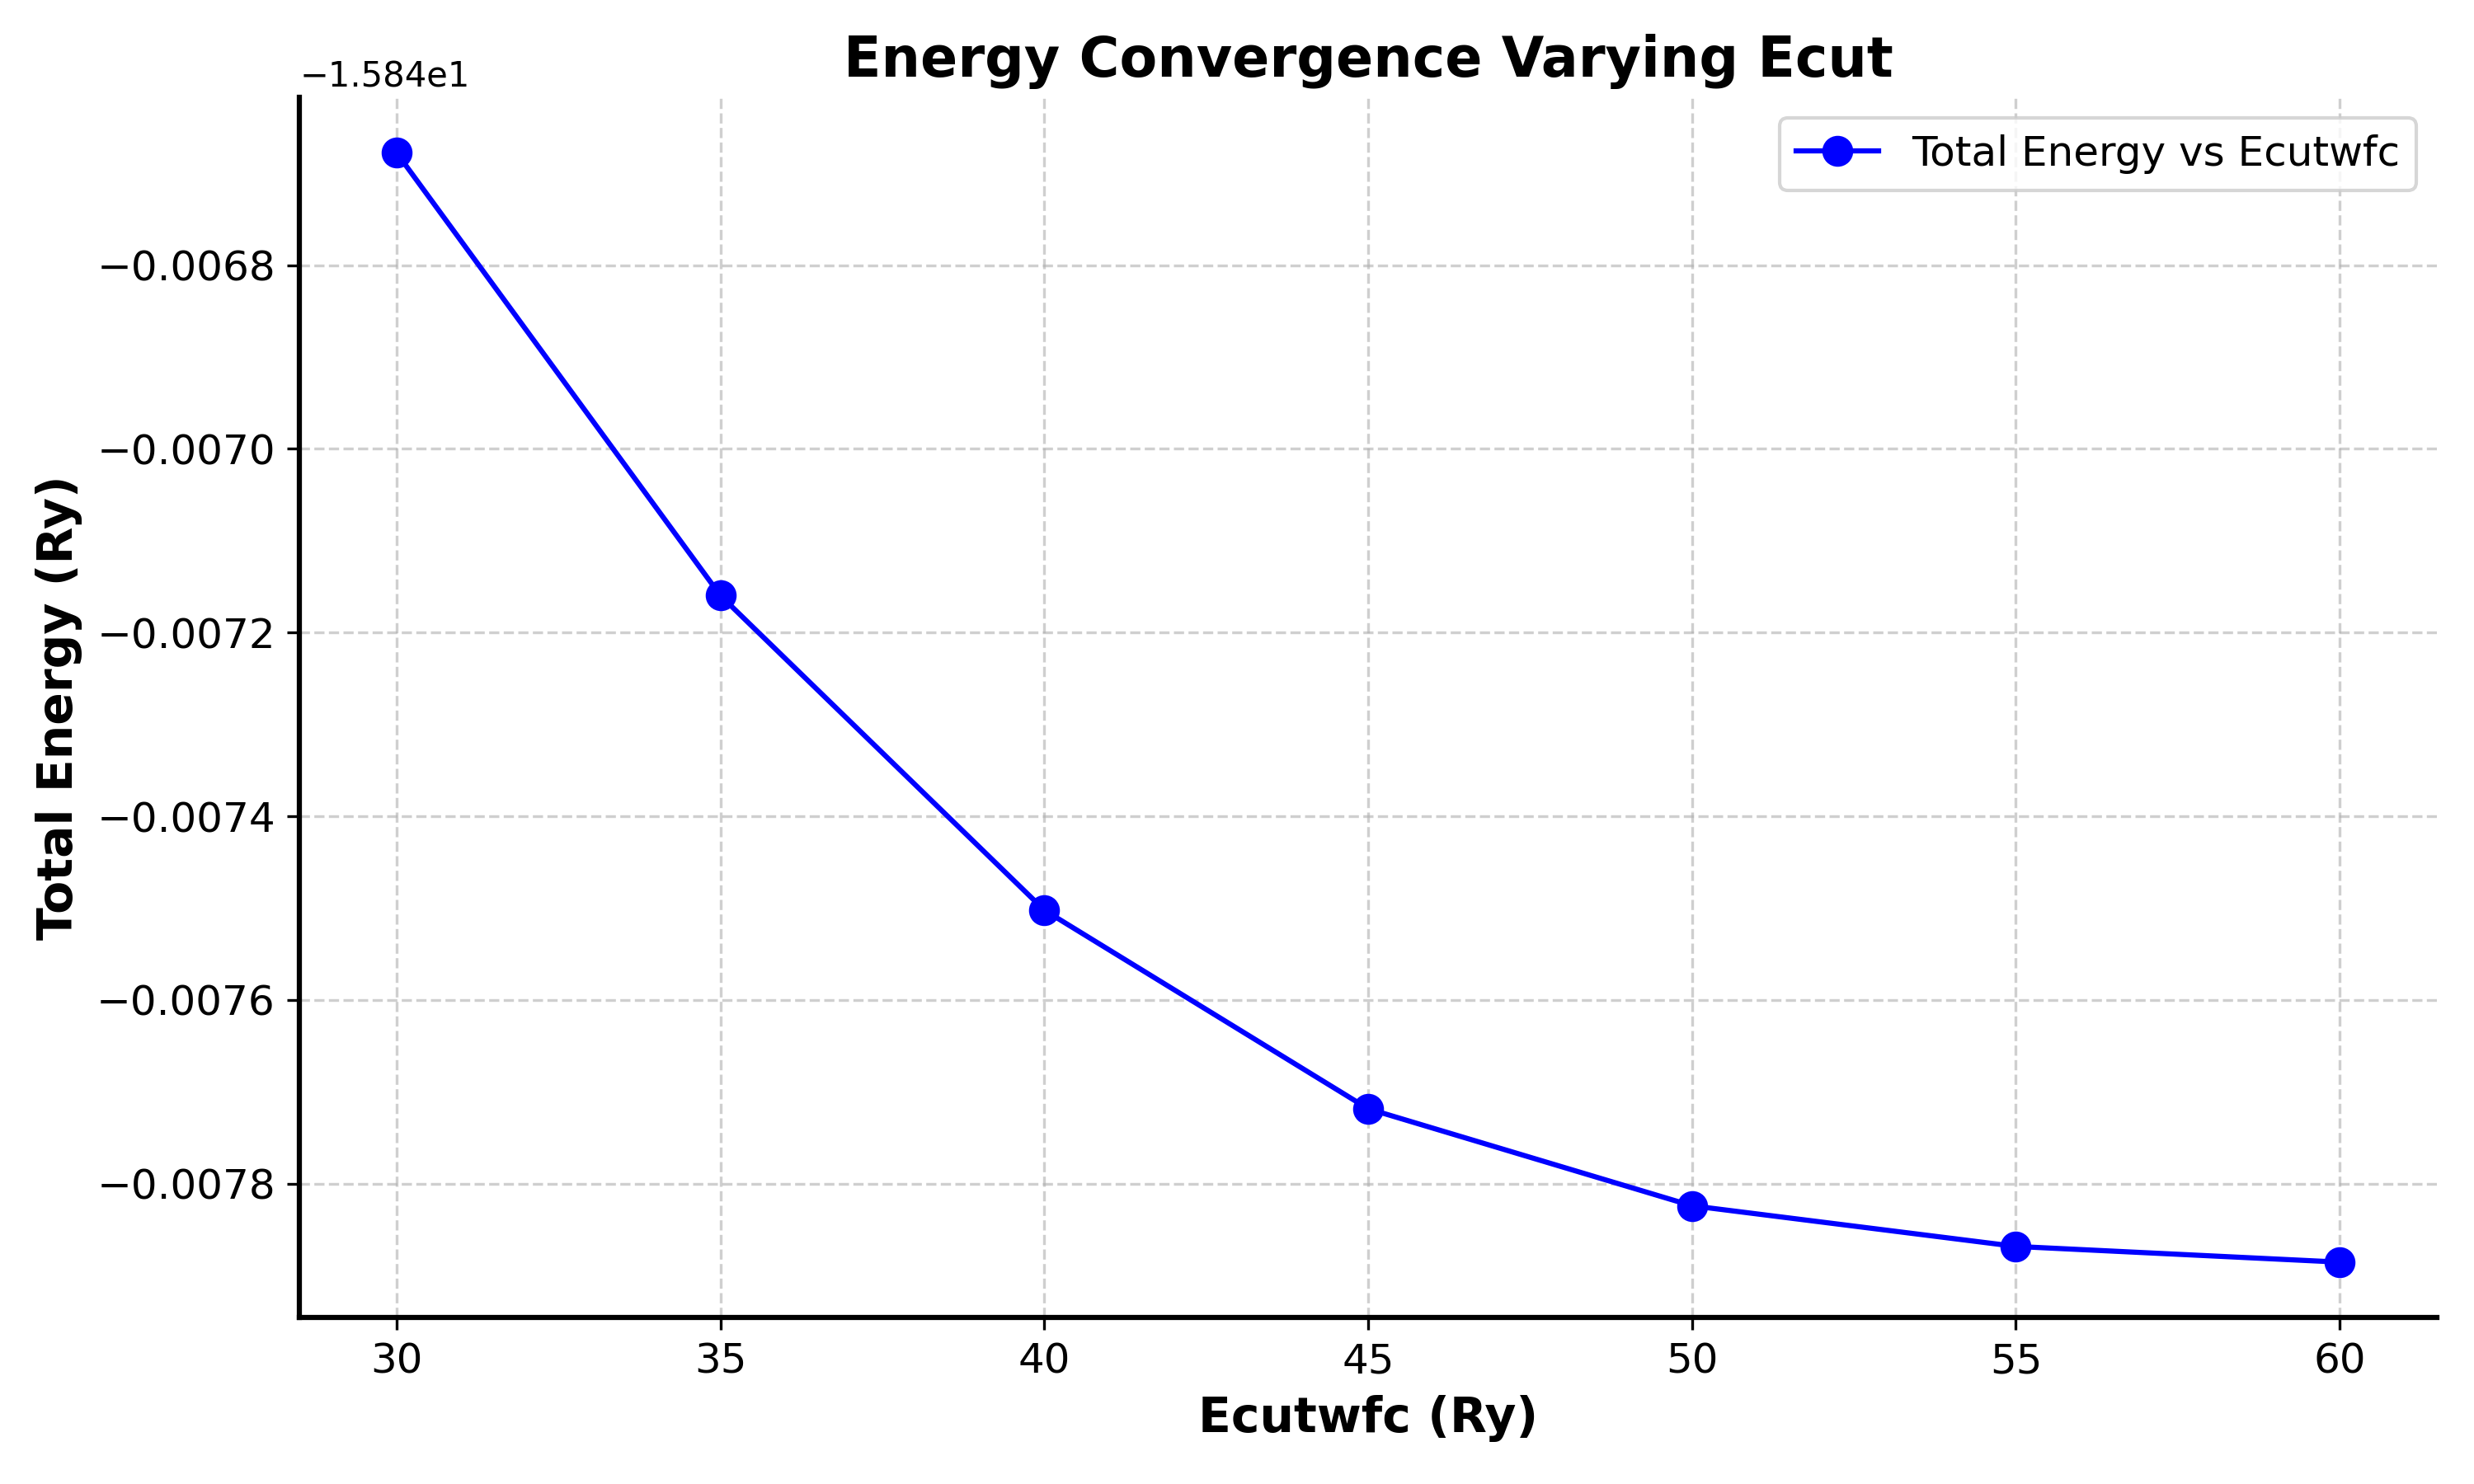
\includegraphics[width=0.7\linewidth]{img/en-ecut_conv_improved.png}
    \caption{Convergence of the total energy of silicon as a function of the kinetic energy cutoff (\verb|ecutwfc|). The energy is shown to stabilize for values above $50$ Ry.}
    \label{fig:en-ecut}
\end{figure}

\begin{figure}[h!]
    \centering
    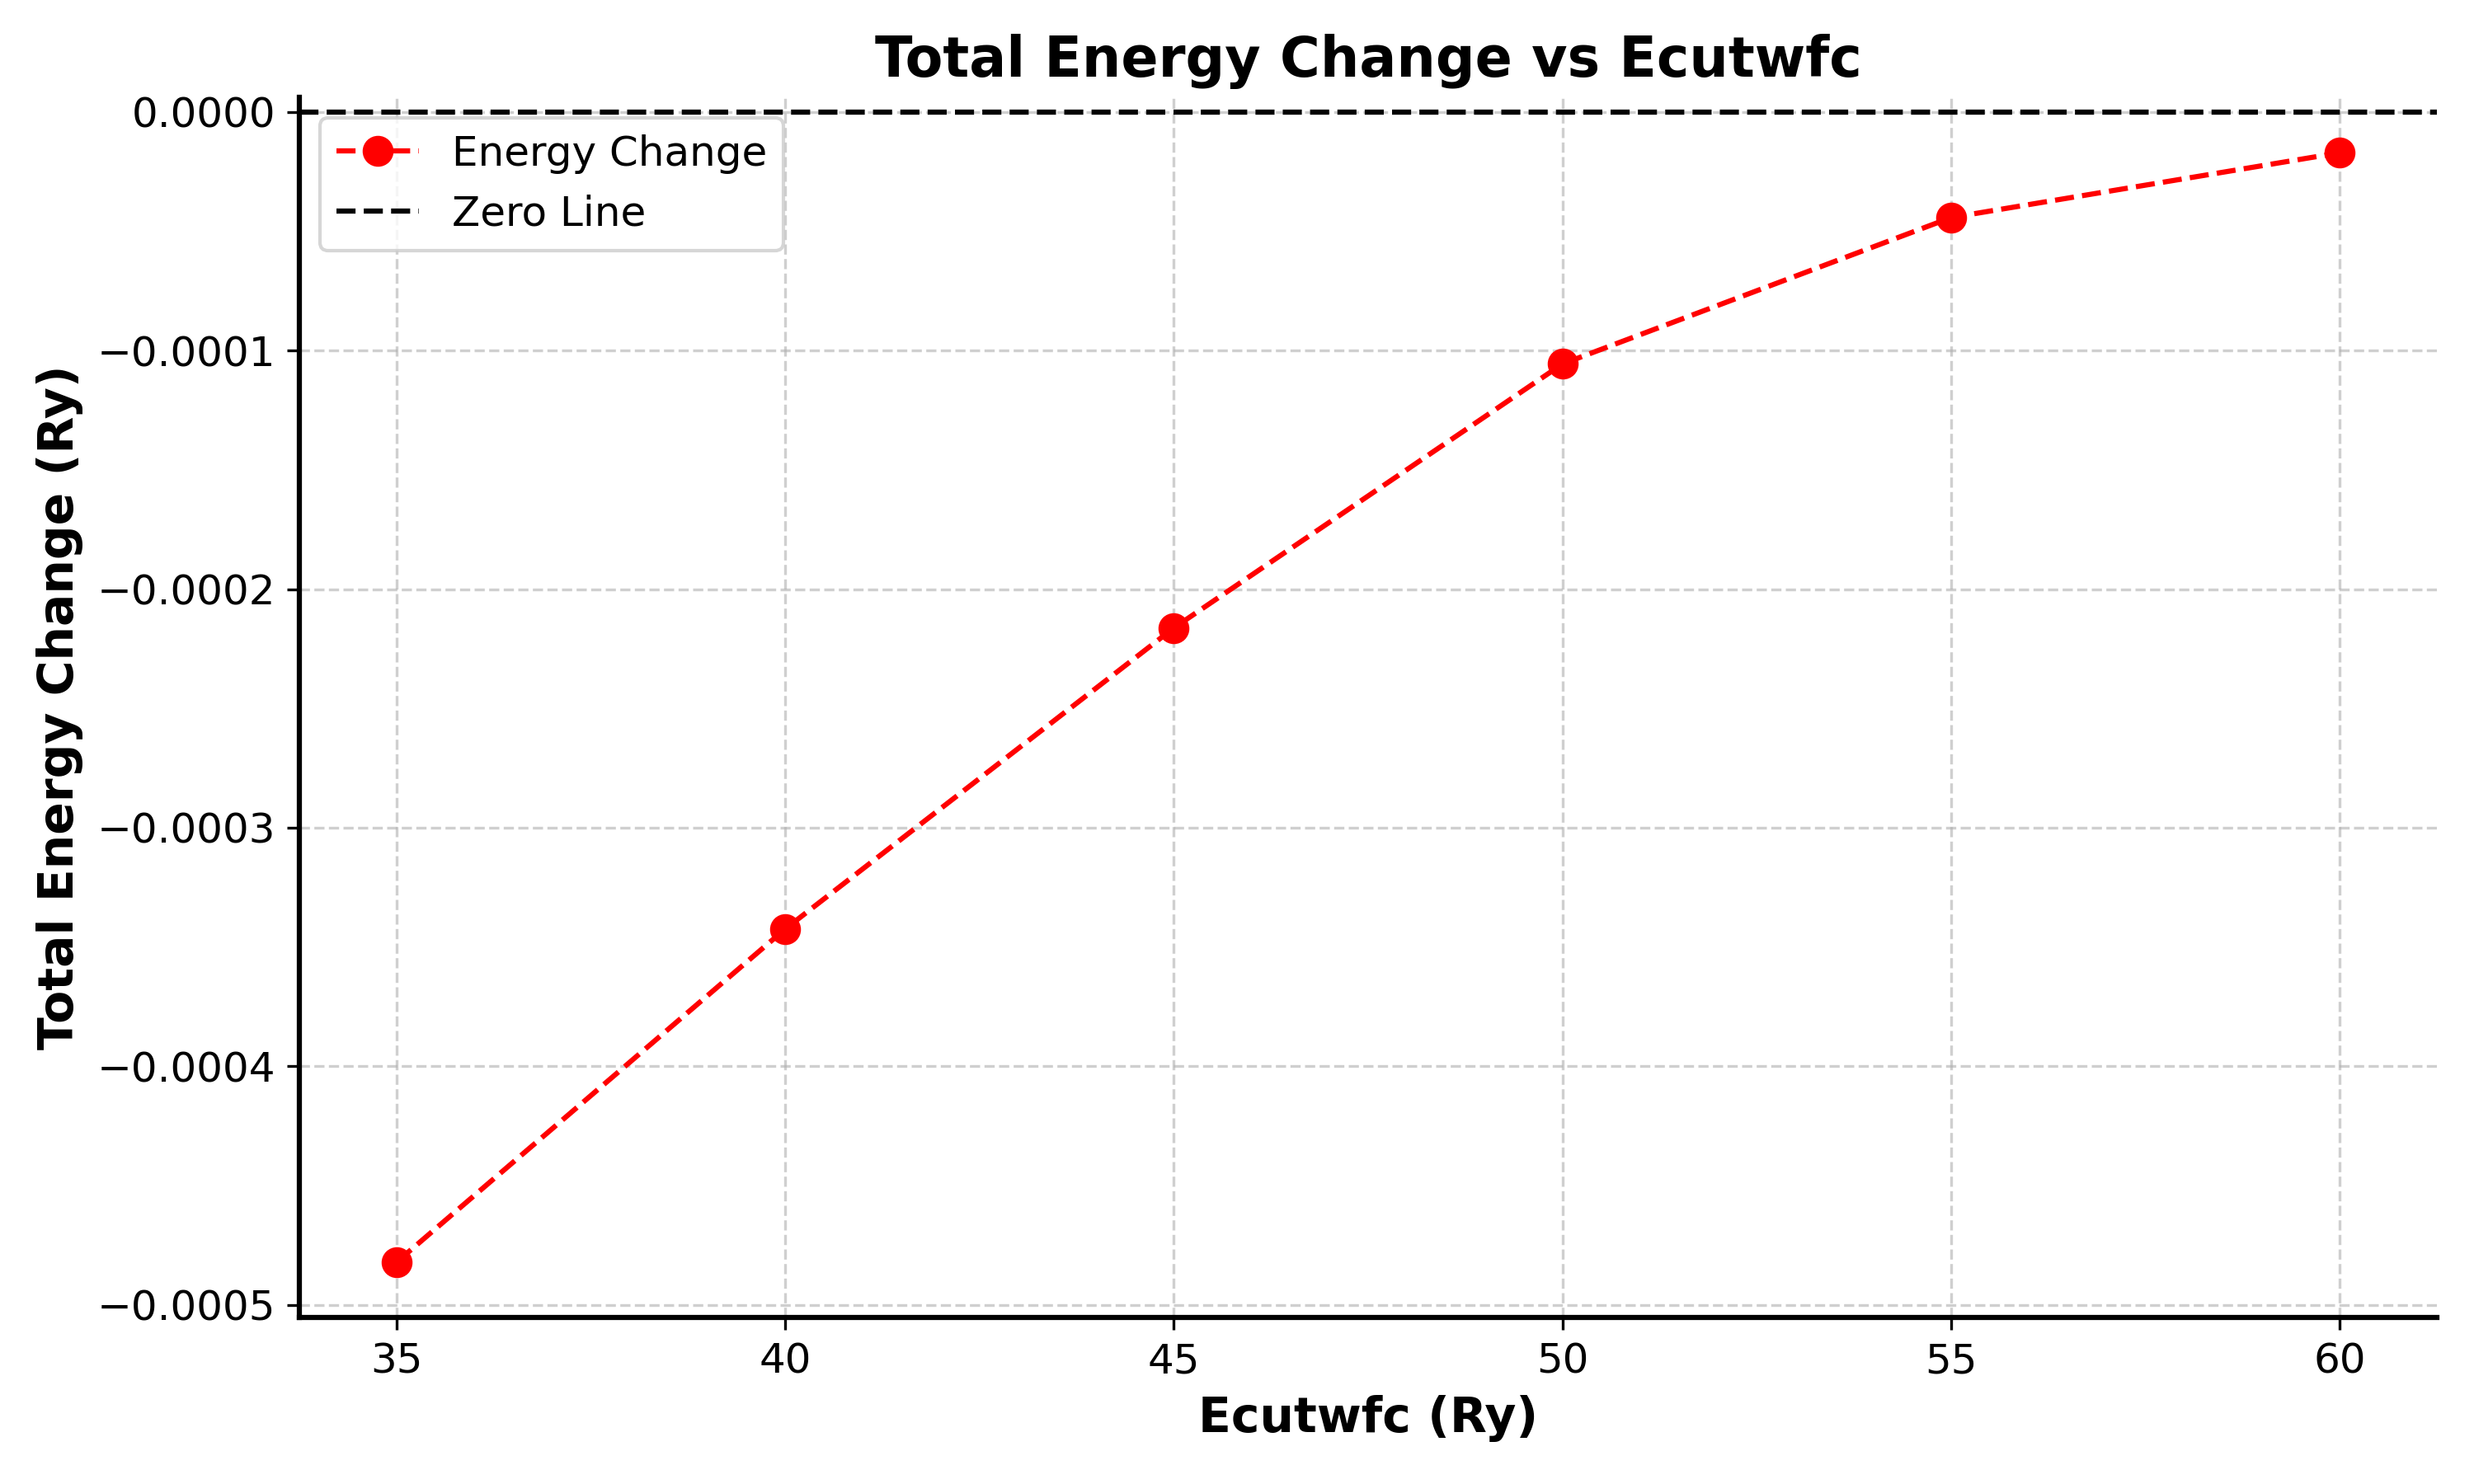
\includegraphics[width=0.7\linewidth]{img/en-ecut_conv_change_improved.png}
    \caption{Energy difference between successive `ecutwfc` values. A convergence threshold of $1$ mRy is reached at $55$ Ry.}
    \label{fig:en-ecut_diff}
\end{figure}

Next, using the converged cutoff of $55$ Ry, we tested the convergence with respect to the k-point mesh density, varying the grid from \verb|3x3x3| to \verb|10x10x10|. Figure \ref{fig:en-kpoint} shows that the total energy is well-converged with a \textbf{\verb|6x6x6|} Monkhorst-Pack grid. Increasing the mesh density further yields negligible changes in energy but significantly increases the computational cost. Therefore, all subsequent calculations were performed using \verb|ecutwfc| = $55$ Ry and a \verb|6x6x6| k-point mesh.

\begin{figure}[h!]
    \centering
    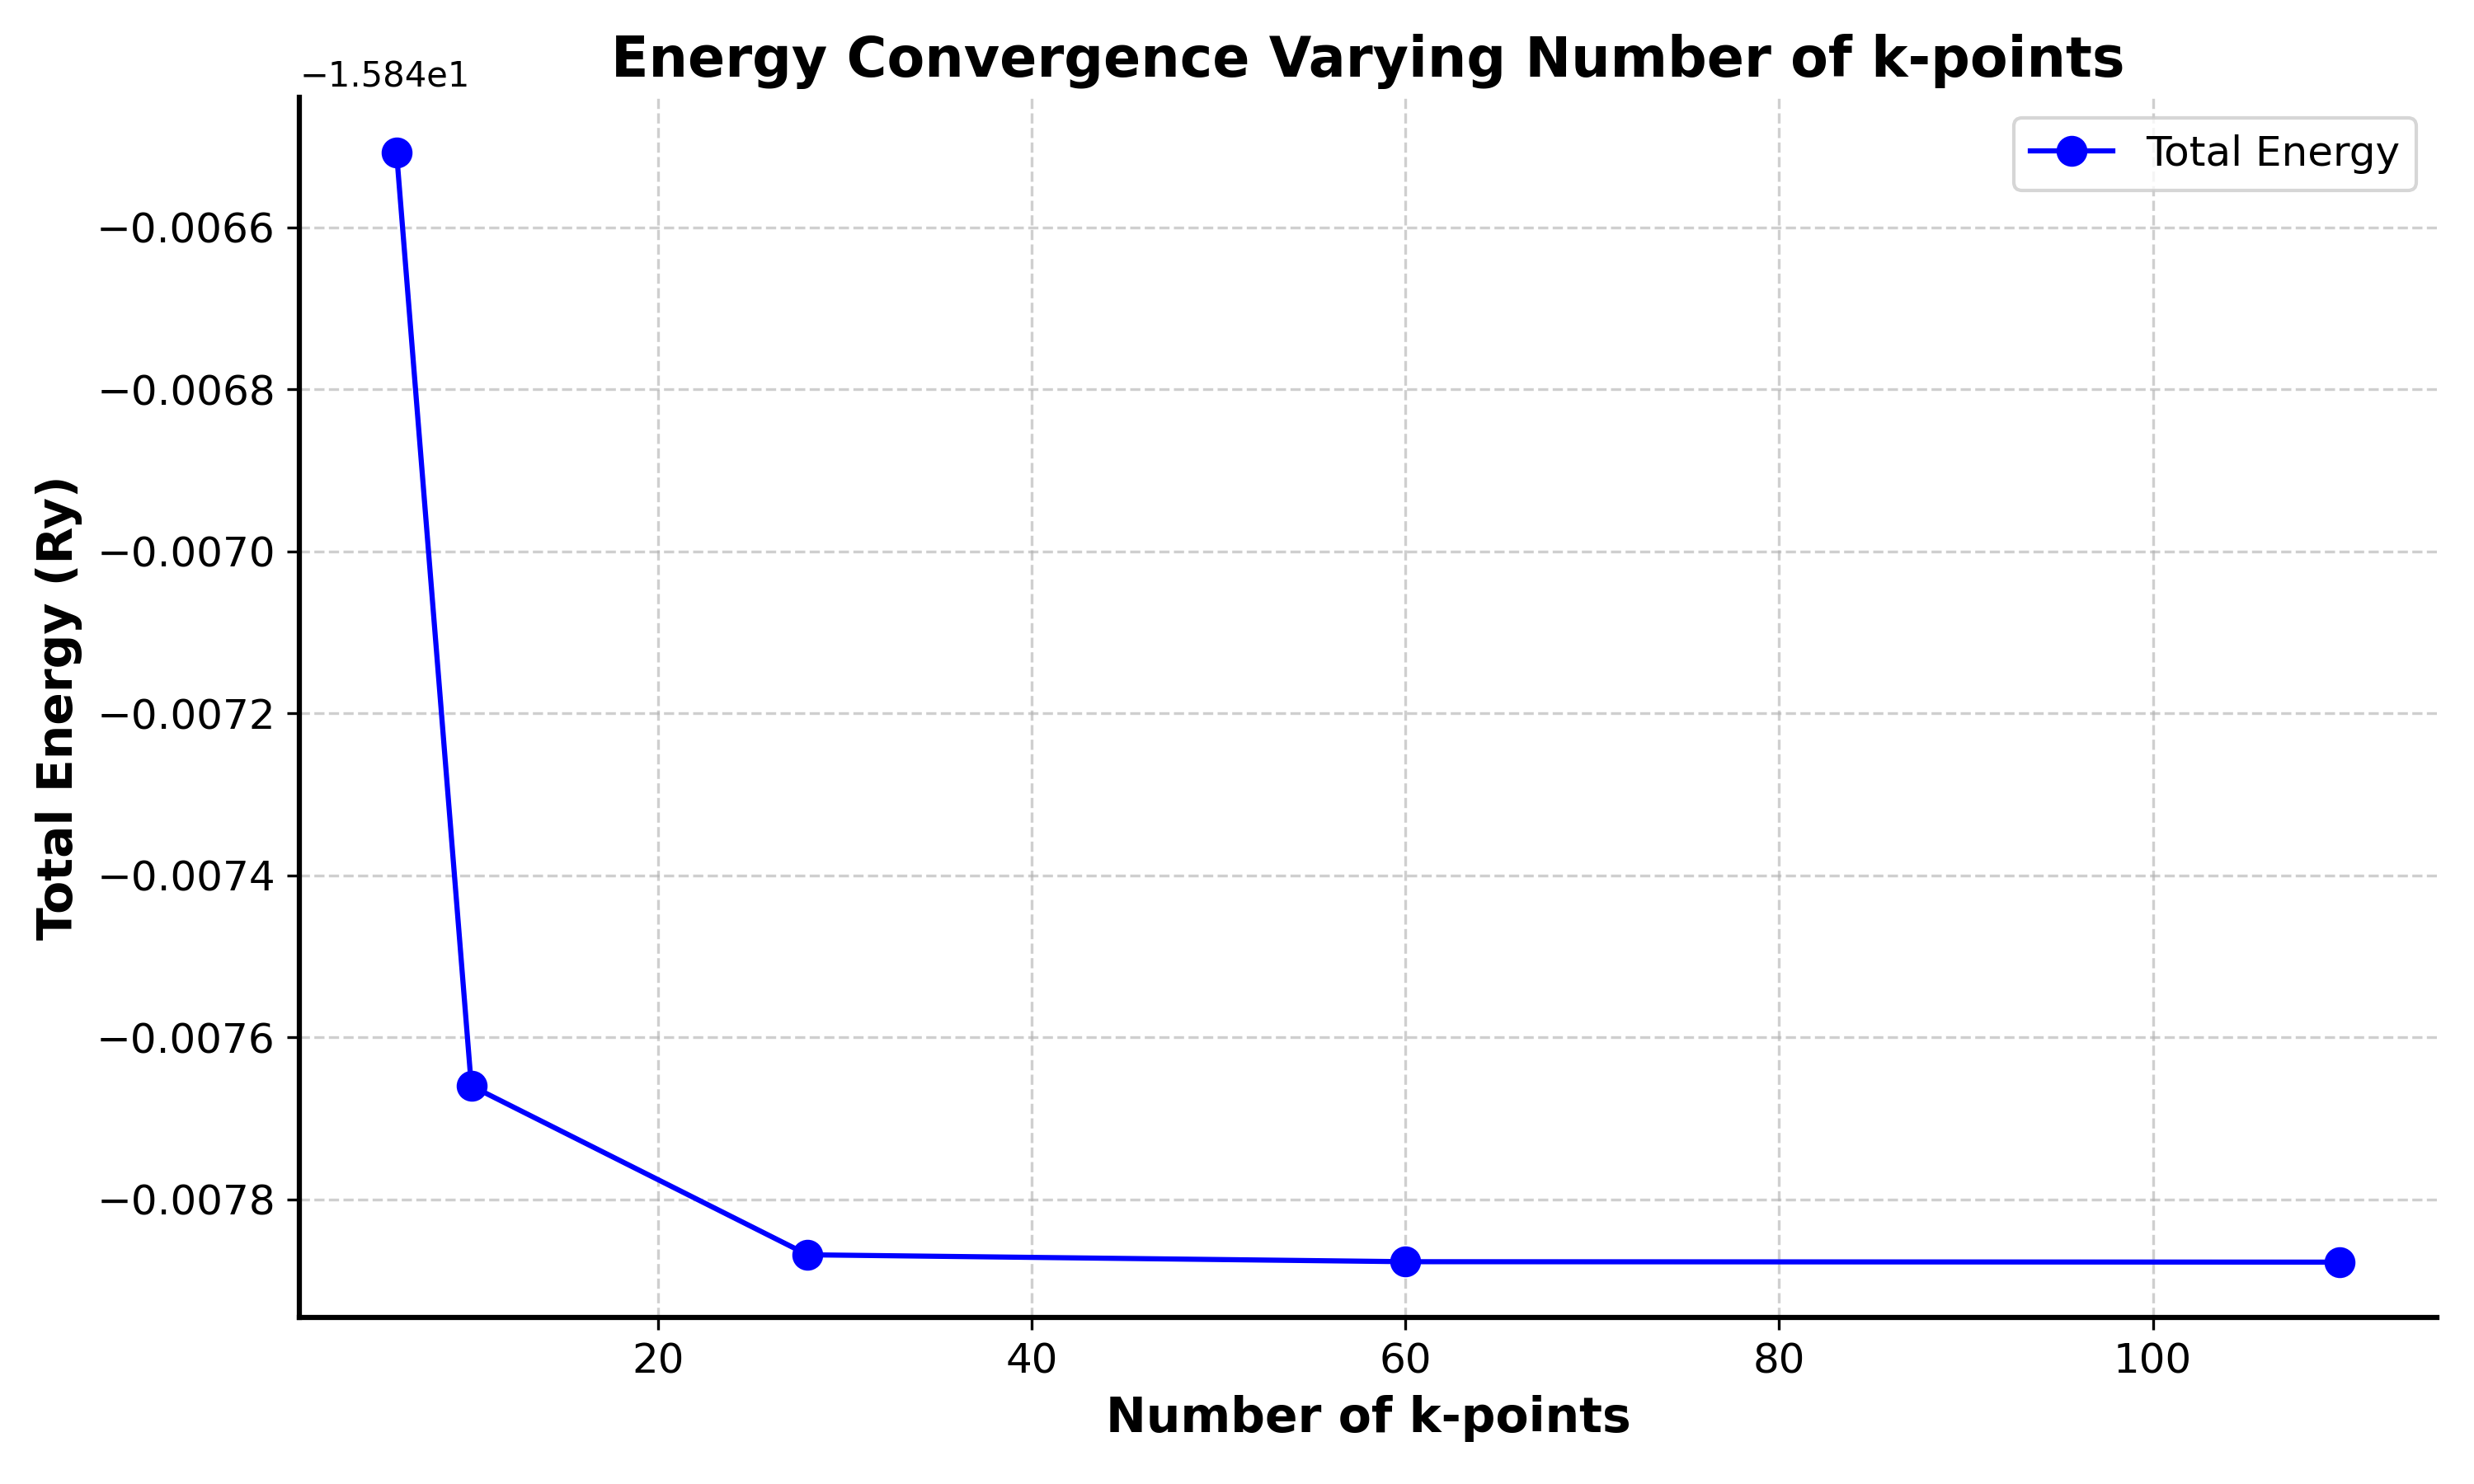
\includegraphics[width=0.7\linewidth]{img/en-kpoint_conv_improved.png}
    \caption{Convergence of the total energy as a function of the k-point mesh density. The energy is converged for a `6x6x6` grid.}
    \label{fig:en-kpoint}
\end{figure}

\subsection{Equation of State and Structural Properties}

With the converged computational parameters established, we calculated the structural properties of silicon at equilibrium. We performed a series of SCF calculations by varying the lattice parameter \verb|a| (\verb|celldm(1)|) from $9.90$ to $10.50$ Bohr, recording the total energy for each corresponding cell volume. The resulting energy-volume data points were then fitted to the Murnaghan equation of state \cite{murnaghan1944}:
$$ E(V) = E_0 + \frac{B_0 V}{B'_0} \left( \frac{(V_0/V)^{B'_0}}{B'_0 - 1} + 1 \right) - \frac{B_0 V_0}{B'_0 - 1} $$
where $E_0$ is the equilibrium energy, $V_0$ is the equilibrium volume, $B_0$ is the bulk modulus, and $B'_0$ is its pressure derivative.

The fitting, performed using the \verb|curve_fit| routine from the \verb|scipy.optimize| library (Fig. \ref{fig:murn}, yielded the equilibrium parameters summarized in Table \ref{tab:eos_results}. Our calculated values are compared with established experimental data.

\begin{figure}[h!]
    \centering
    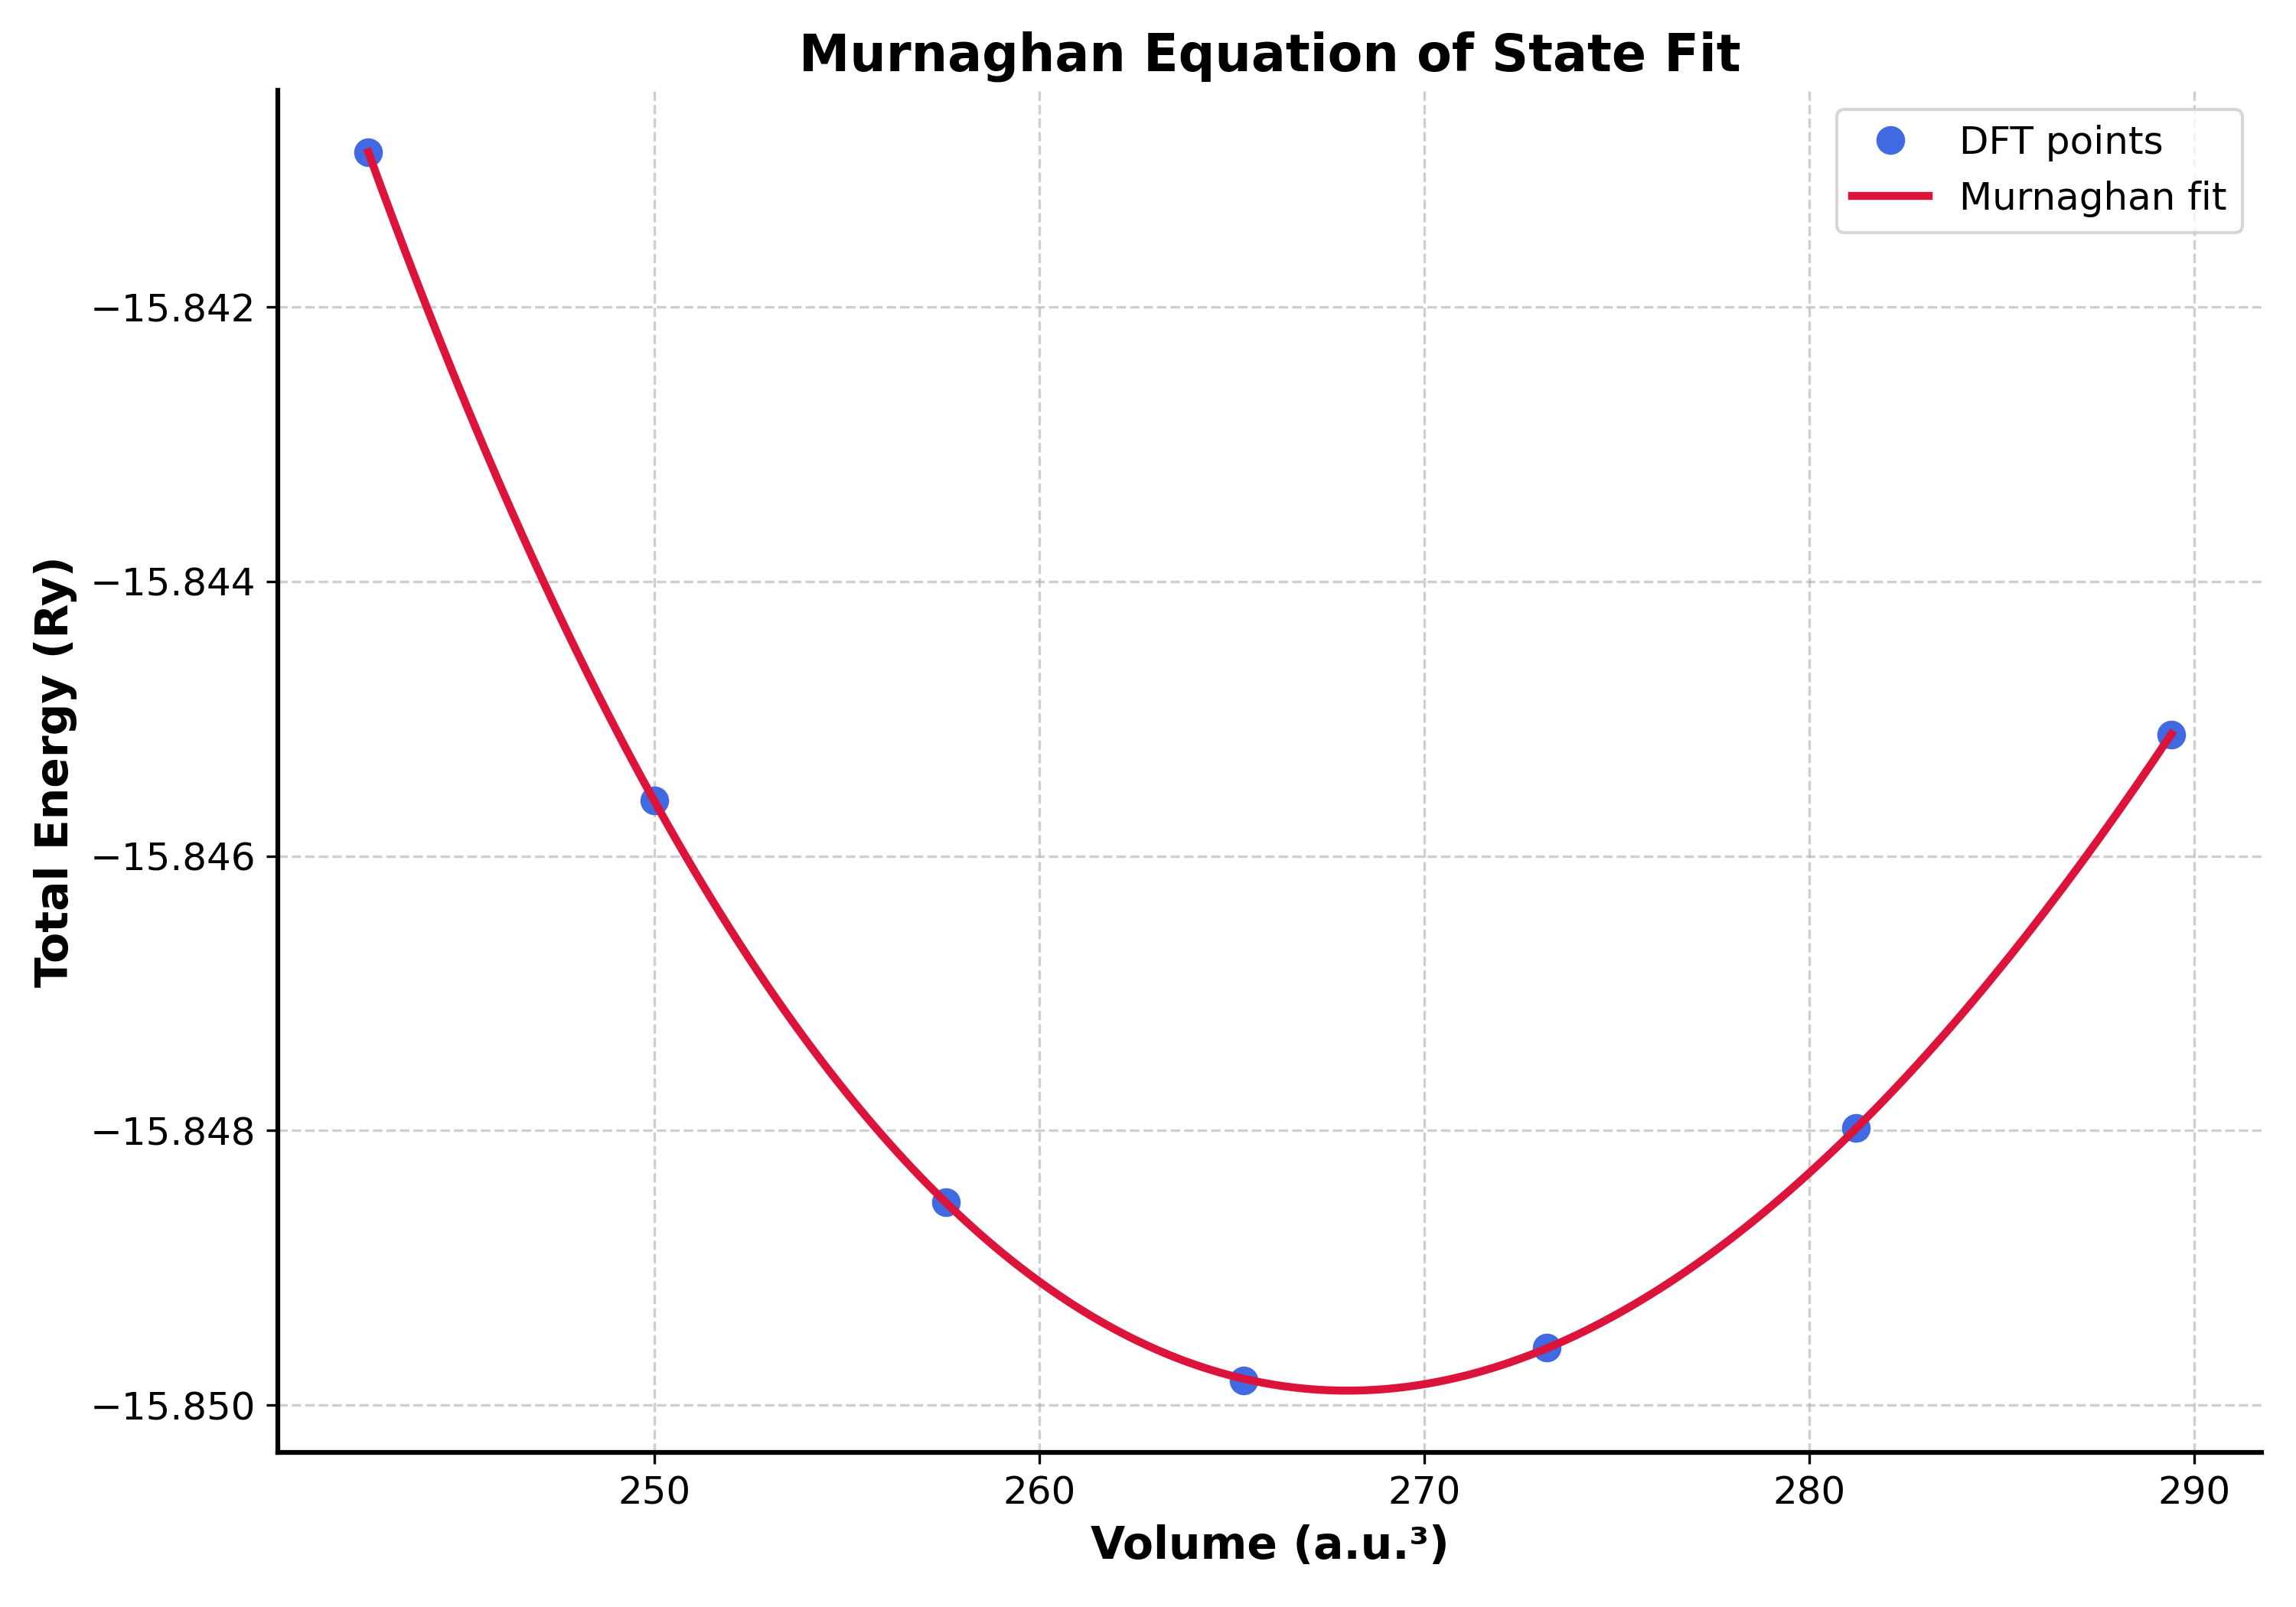
\includegraphics[width=0.7\linewidth]{img/murnaghan_fit_improved.png}
    \caption{Plot of total energy versus volume. The blue circles are the DFT calculated data points, and the red line is the fit using the Murnaghan equation of state.}
    \label{fig:murn}
\end{figure}

\begin{table}[h!]
    \centering
    \caption{Calculated structural properties of silicon compared with experimental values.}
    \label{tab:eos_results}
    \begin{tabular}{l c c}
        \hline\hline
        \textbf{Property} & \textbf{Calculated (PBE)} & \textbf{Experimental} \\
        \hline
        Lattice constant, $a_0$ (\AA) & $5.416$ & $5.431$ \cite{okada1984} \\
        Bulk modulus, $B_0$ (GPa) & $93.3$ & $98$ \cite{Junquera2001} \\
        Equilibrium energy, $E_0$ (Ry/atom) & $-7.925$ & - \\
        Equilibrium volume, $V_0$ (a.u.$^3$/atom) & $134.0$ & - \\
        $B'_0$ & $3.92$ & $\sim 4.2$ \cite{Junquera2001} \\
        \hline\hline
    \end{tabular}
\end{table}

The results show excellent agreement with the experimental data. Our calculated lattice constant of $a_0 = 5.416$~\AA\ has a relative error of only $-0.28\%$ compared to the experimental value. This slight underestimation of the lattice parameter and a corresponding slight underestimation of the bulk modulus ($B_0 = 93.3\sim$ GPa vs. $98$ GPa) are well-known and typical results for the PBE functional when applied to covalently bonded semiconductors like silicon \cite{haas2009}. The high level of accuracy confirms the validity of our computational setup and provides a solid foundation for the subsequent analysis of electronic and vibrational properties.

%Osservazioni dal Grafico convergenza:

%Andamento Corretto: L'energia totale diminuisce all'aumentare di ecutwfc. Questo è l'andamento atteso, poiché una base di onde piane più grande (maggiore ecutwfc) permette una descrizione variazionale migliore dello stato fondamentale, portando a un'energia più bassa (più negativa).
%Convergenza Visibile: La curva si sta chiaramente appiattendo verso valori più alti di ecutwfc. La pendenza della curva diminuisce significativamente dopo i 45-50 Ry.
%Valori sull'asse Y: L'asse Y mostra valori intorno a -15.84 Ry, e poi si concentra sulla variazione decimale (da -0.0067 a -0.0079 Ry circa, rispetto a -15.8400 Ry). Questo significa che stiamo osservando variazioni dell'ordine di 0.001 Ry.




%Analisi del Grafico "Total Energy Change vs Ecutwfc Index":

%Asse X (Ecutwfc Index): Questo asse rappresenta i tuoi diversi valori di ecutwfc in ordine crescente.
%Indice 1 potrebbe corrispondere a 30 Ry, Indice 2 a 35 Ry, ..., Indice 6 a 55 Ry (se il penultimo punto è 55 Ry) o a 60 Ry (se l'ultimo punto è 60 Ry). Dobbiamo capire a quale ecutwfc si riferisce l'indice per essere precisi.
%Asse Y (Total Energy Change (Ry)): Mostra quanto cambia l'energia. La "Zero Line" rossa tratteggiata è il riferimento, idealmente la convergenza è raggiunta quando i punti si avvicinano molto a questa linea (cioè, l'energia non cambia più significativamente aumentando ulteriormente ecutwfc).
%Andamento dei Punti:
%I primi punti (Indice 1, 2, 3) mostrano una variazione di energia ancora relativamente grande (dell'ordine di -0.0005 Ry, -0.00035 Ry, -0.0002 Ry).
%Il punto all'Indice 4 mostra una variazione di circa -0.0001 Ry.
%Il punto all'Indice 5 mostra una variazione molto piccola, forse intorno a -0.00005 Ry o meno.
%Il punto all'Indice 6 è ancora più vicino allo zero, indicando una variazione quasi trascurabile.
%Interpretazione in termini di ecutwfc (ipotizzando che l'Indice 1 = 30 Ry, Indice 2 = 35 Ry, ..., Indice 6 = 55 Ry):

%Indice 4 (corrisponderebbe a 45 Ry): ΔE ≈ -0.0001 Ry. Ricordando che il nostro criterio di ~1 meV/atomo è circa 0.000147 Ry/cella, questo valore è già buono.
%Indice 5 (corrisponderebbe a 50 Ry): ΔE < 0.00005 Ry. Ottima convergenza.
%Indice 6 (corrisponderebbe a 55 Ry): ΔE ancora più piccola, eccellente convergenza.
%Se l'ultimo punto (Indice 6) corrisponde a 60 Ry (e quindi l'Indice 5 a 55 Ry, l'Indice 4 a 50 Ry, ecc.), allora:

%Indice 4 (50 Ry): ΔE ≈ -0.0001 Ry. Buona convergenza.
%Indice 5 (55 Ry): ΔE < -0.00005 Ry (difficile da leggere ma molto piccola). Ottima convergenza.
%Indice 6 (60 Ry): ΔE quasi a zero. Eccellente convergenza.












\section{Band Structure of Silicon}

The electronic band structure and the energy gap are fundamental material properties that determine the electronic and optical behavior of semiconductors.

We start by initializing a \verb|scf.in| file where we define the unit cell as before, using the parameters previously computed: \verb|celldm(1) = 10.234422| bohr and \verb|ecutwfc = 55| Ry. The calculation employs the LDA (Local Density Approximation) exchange-correlation functional with norm-conserving pseudopotentials. We specify the location of two Si atoms at positions $(0,0,0)$ and $(0.25,0.25,0.25)$ in crystal coordinates, corresponding to the diamond structure. The \verb|K-POINT| grid is set to $12\times12\times12$ with a Monkhorst-Pack scheme to ensure accurate sampling of the Brillouin zone for the subsequent non-self-consistent calculation.

First, we perform a self-consistent field (SCF) calculation to compute the electronic density for the ground state with a convergence threshold of $10^{-8}$ Ry. With the converged charge density, we perform a non-self-consistent field (NSCF) calculation using the \verb|bands| keyword. This calculation computes $16$ bands (\verb|nbnd=16|), consisting of $4$ valence bands (fully occupied, containing 8 electrons) and $12$ conduction bands (empty), which is appropriate for silicon with $8$ valence electrons per unit cell.

At this point, we prepare the input file for the post-processing using \verb|bands.x|. We define a path through high-symmetry points in the FCC Brillouin zone following the standard notation:
$$
\Gamma \rightarrow \text{X} \rightarrow \text{W} \rightarrow \text{K} \rightarrow \Gamma \rightarrow \text{L} \rightarrow \text{U} \rightarrow \text{W} \rightarrow \text{L} \rightarrow \text{K}
$$
where $\Gamma = (0,0,0)$, $\text{X} = (0.5,0,0.5)$, $\text{W} = (0.5,0.25,0.75)$, $\text{K} = (0.375,0.375,0.75)$, $\text{L} = (0.5,0.5,0.5)$, and $\text{U} = (0.625,0.25,0.625)$ in crystal coordinates. We use $40$ points between each pair of high-symmetry points to ensure smooth band dispersion curves.

Using a Python script with the \verb|numpy| library for data processing, we analyze the output to determine:
\begin{itemize}
    \item Valence band maximum (VBM) = $6.123$ eV at the $\Gamma$ point
    \item Conduction band minimum (CBM) = $7.133$ eV along the $\Gamma$-X direction
\end{itemize}

From these values, we calculate the indirect band gap:
\begin{equation}
E_g = \text{CBM} - \text{VBM} = 1.010 \text{ eV}
\end{equation}

We visualize the band structure in Fig.~\ref{fig:band_structure}, plotting the valence bands in blue and the conduction bands in red. The energy scale is normalized such that the VBM is set to $0$~eV, and the high-symmetry points are marked along the x-axis. The band structure clearly shows:
\begin{itemize}
    \item Silicon has an indirect band gap, with the VBM at $\Gamma$ and the CBM along the $\Gamma$-X direction.
    \item The direct gap at $\Gamma$ is approximately $2.6\sim$ eV.
    \item The valence bands show the characteristic degeneracy at the $\Gamma$ point, which is lifted along other directions due to crystal symmetry.
\end{itemize}

The calculated band gap of $1.010\sim$eV is in good agreement with, though slightly lower than, the experimental value of $1.17\sim$ eV at low temperature \cite{green1990}. This underestimation of approximately $14\%$ is a well-known limitation of DFT with local or semi-local exchange-correlation functionals, which fail to properly account for the derivative discontinuity of the exchange-correlation potential \cite{perdew2017}. Despite this quantitative discrepancy, the band structure topology and the indirect nature of the gap are correctly reproduced, confirming that silicon is an indirect gap semiconductor with the conduction band minimum located at approximately $0.85\times(2\pi/a)$ along the $\Gamma$-X direction \cite{chelikowsky1976}.

\begin{figure}[h!]
    \centering
    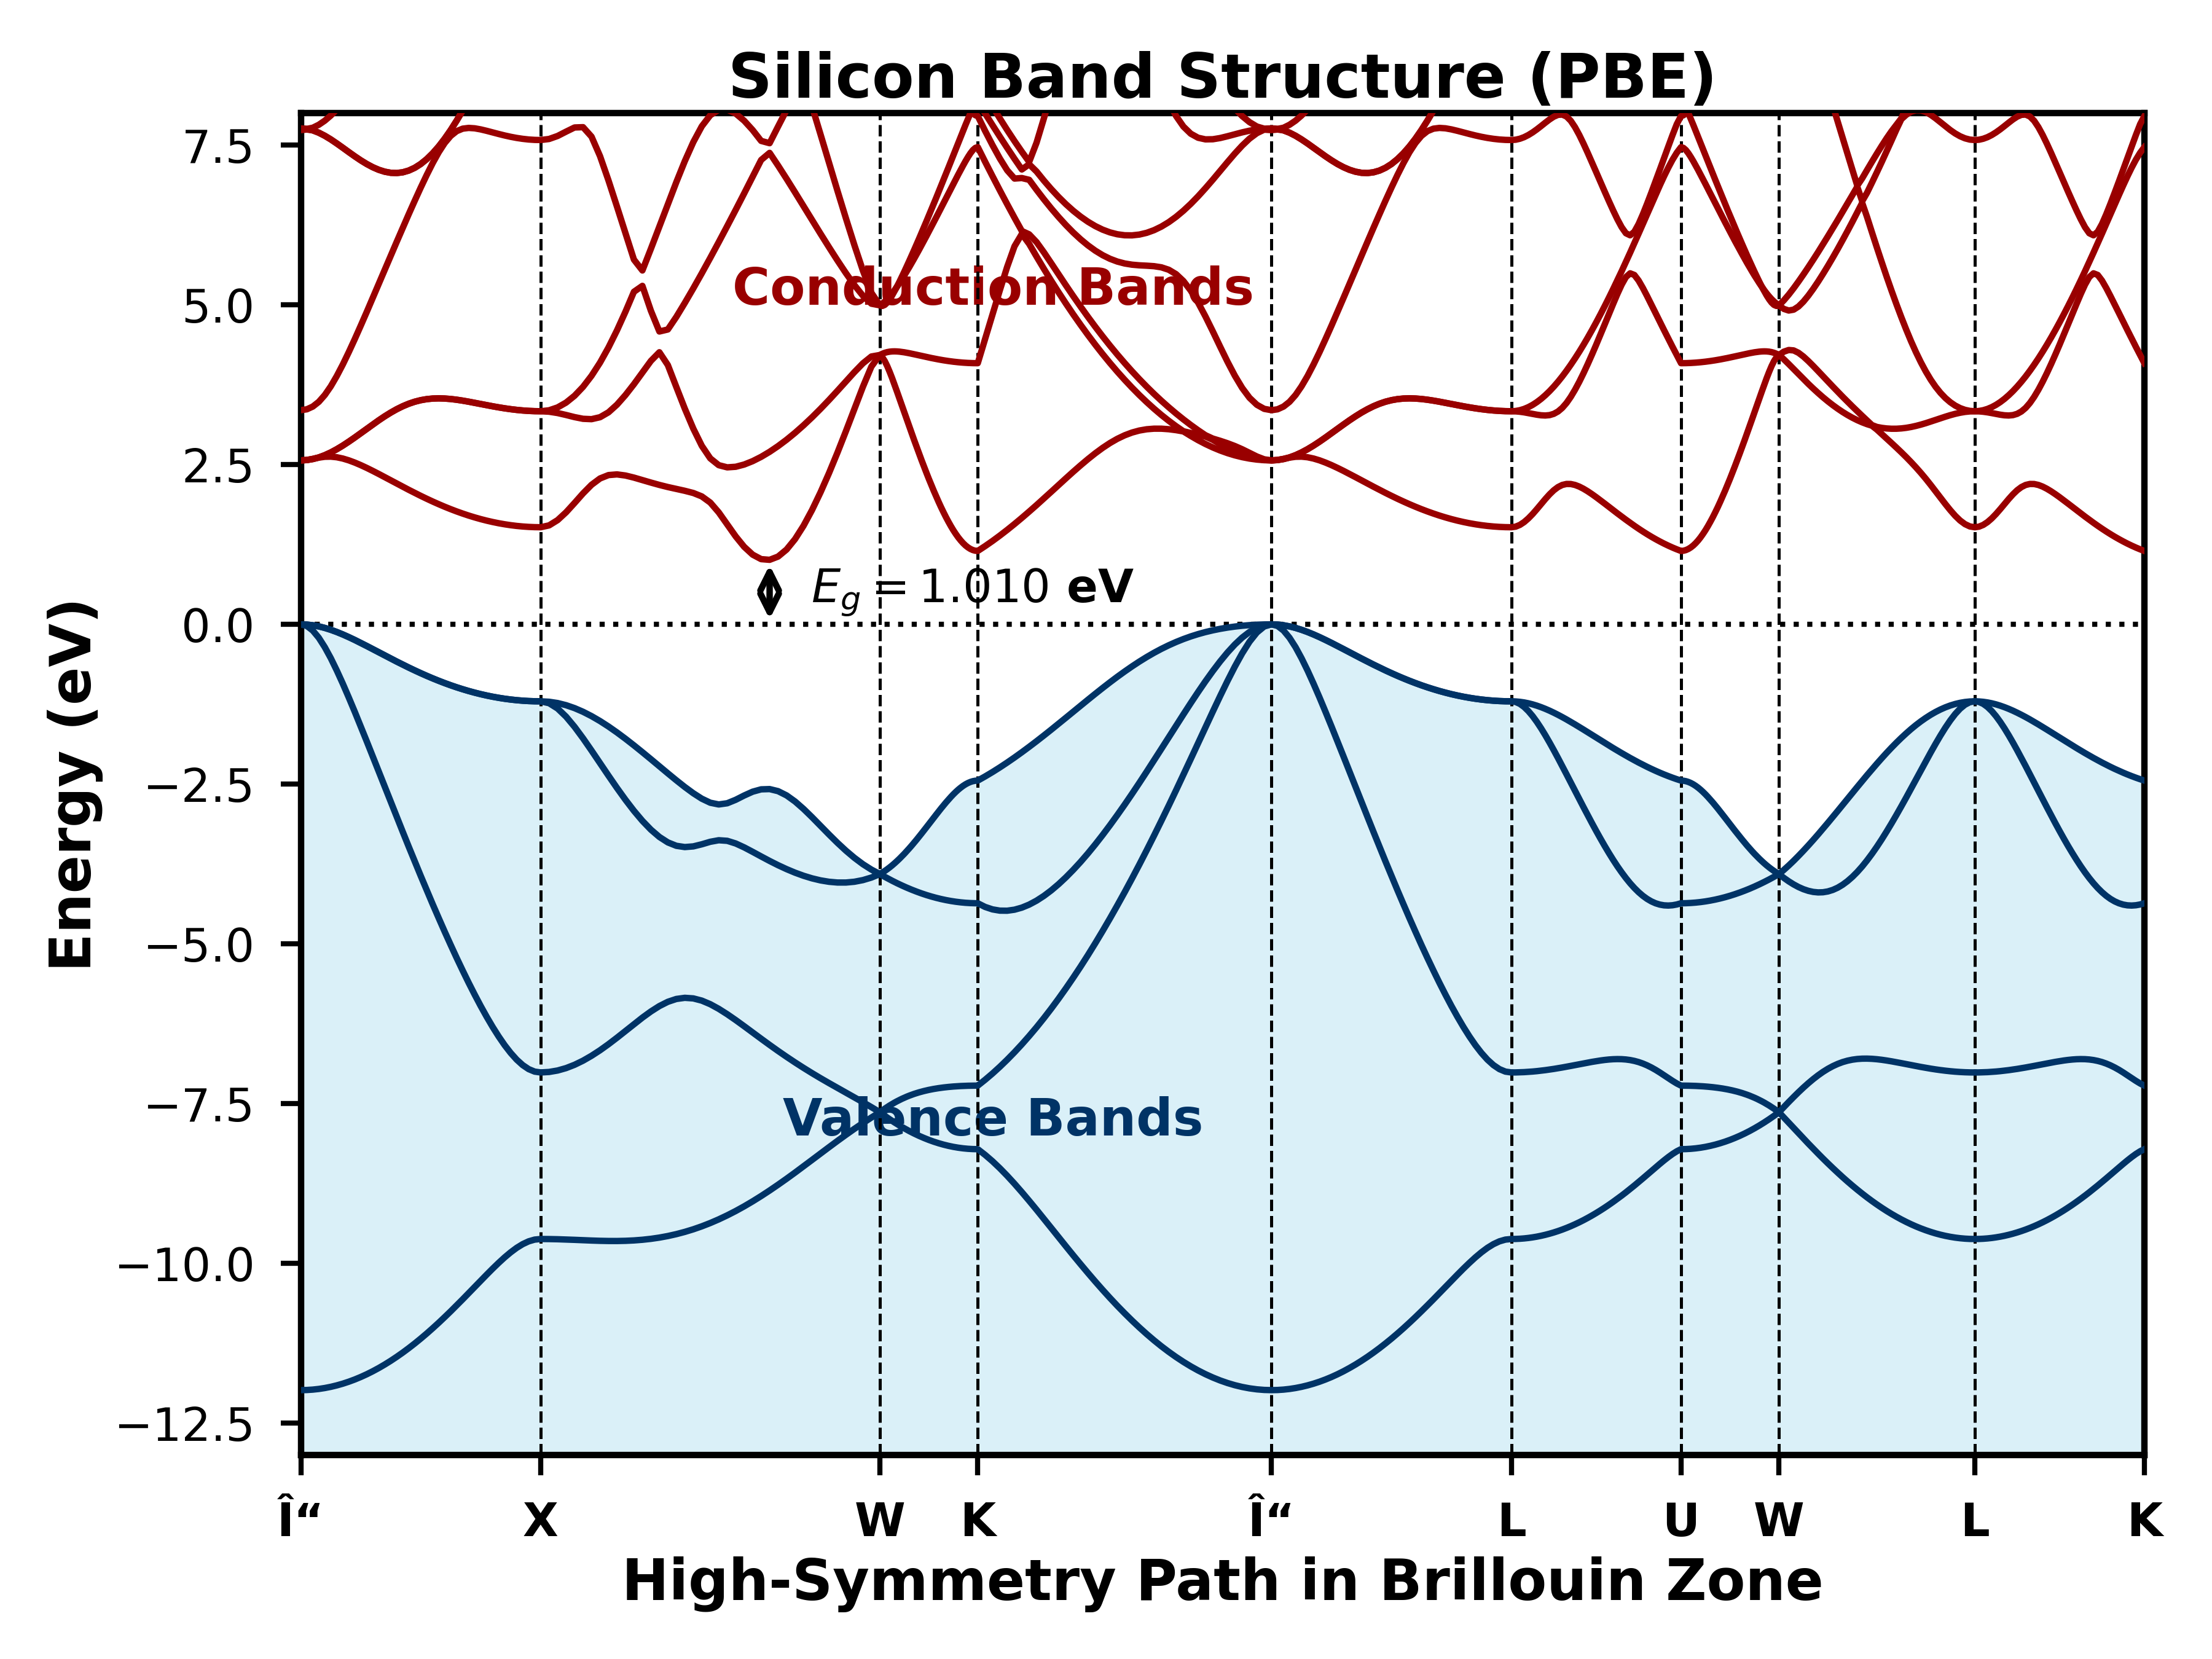
\includegraphics[width=0.8\textwidth]{img/silicon_band_structure_final.png} % Assicurati che il nome del file sia corretto
    \caption{Calculated electronic band structure of silicon. The valence bands are shown in blue and conduction bands in red. The energy is referenced to the valence band maximum (VBM).}
    \label{fig:band_structure}
\end{figure}


%I)dentificazione della natura indiretta del gap di banda del silicio
%Il VBM si trova al punto Γ
%Il CBM si trova lungo la direzione Γ-X
%Gap di banda calcolato: 0.635 eV (inferiore al valore sperimentale di ~1.1-1.2 eV, una sottostima tipica dei calcoli DFT con funzionali standard)
%Confronto con i dati sperimentali:

%Il gap calcolato è sottostimato rispetto al valore sperimentale (~1.1-1.2 eV)
%Questa sottostima è una limitazione nota dei calcoli DFT con funzionali LDA/GGA
%La struttura generale delle bande è comunque in accordo qualitativo con i dati sperimentali
%Conclusioni
%Il calcolo ha prodotto con successo la struttura a bande del silicio cristallino, mostrando correttamente la sua natura di semiconduttore a gap indiretto. Il gap di banda calcolato (0.635 eV) è coerente con i risultati tipici ottenuti con calcoli DFT standard, che tendono a sottostimare il gap. La visualizzazione della struttura a bande mostra chiaramente la separazione tra le bande di valenza e di conduzione, permettendo un'analisi dettagliata delle proprietà elettroniche del materiale.

%Il file più adatto come template di partenza è si-scf (o si-scf_1).

%Primo passo: Test di convergenza.
%Convergenza ecutwfc: Partendo da si-scf, fissa i K_POINTS (ad esempio, a 6 6 6 1 1 1 o 8 8 8 1 1 1, che sono più ragionevoli di 3 3 3 per il Si) e celldm(1) (ad es. 10.2 Bohr, più vicino al valore atteso). Esegui una serie di calcoli scf aumentando ecutwfc (es. 20, 25, 30, 35, 40, 45, 50 Ry) e osserva quando l'energia totale converge.
%Convergenza k-points: Una volta scelto ecutwfc, fissalo. Esegui una serie di calcoli scf variando la griglia di k-point (es. 3 3 3 1 1 1, 4 4 4 1 1 1, 6 6 6 1 1 1, 8 8 8 1 1 1, 10 10 10 1 1 1) e osserva la convergenza dell'energia totale.


\section{Density of Electronic States of Silicon}

The Density of Electronic States (DOS) represents a fundamental property useful for understanding the electronic behavior of materials \cite{ashcroft_mermin_1976}. The DOS of the Si diamond structure was computed using Density Functional Theory (DFT) as implemented in Quantum ESPRESSO. This study complements the previous band structure analysis, providing further information about the electronic properties of silicon.

The DOS has been computed following a three-step approach:
\begin{itemize}
    \item \textbf{Self-consistent calculation (SCF):} Using the parameters from the structural optimization, we first calculated the ground state electronic density on a $12\times12\times12$ k-point grid.
    \item \textbf{Non-self-consistent calculation (NSCF):} The charge density from the SCF step was used as input for a subsequent calculation on a denser k-point grid to obtain highly-resolved eigenvalues.
    \item \textbf{DOS calculation:} Using the \verb|dos.x| post-processing module, the density of electronic states was computed from the NSCF results. We set the energy range from $-15.0\sim$ eV to $10.0\sim$ eV with an energy resolution (\verb|DeltaE|) of $0.02\sim$ eV.
\end{itemize}

A Python script was then used to process and visualize the data. To obtain a continuous and smooth representation of the DOS while preserving its physical features, a Savitzky-Golay filter \cite{savitzky_golay_1964} was applied to the raw data, as shown in Fig. \ref{fig:dos}. The energy scale is shifted such that the Fermi level ($E_F$), which corresponds to the Valence Band Maximum (VBM) in a semiconductor at $0\sim$ K, is set to $0\sim$ eV.

\begin{figure}[h!]
    \centering
    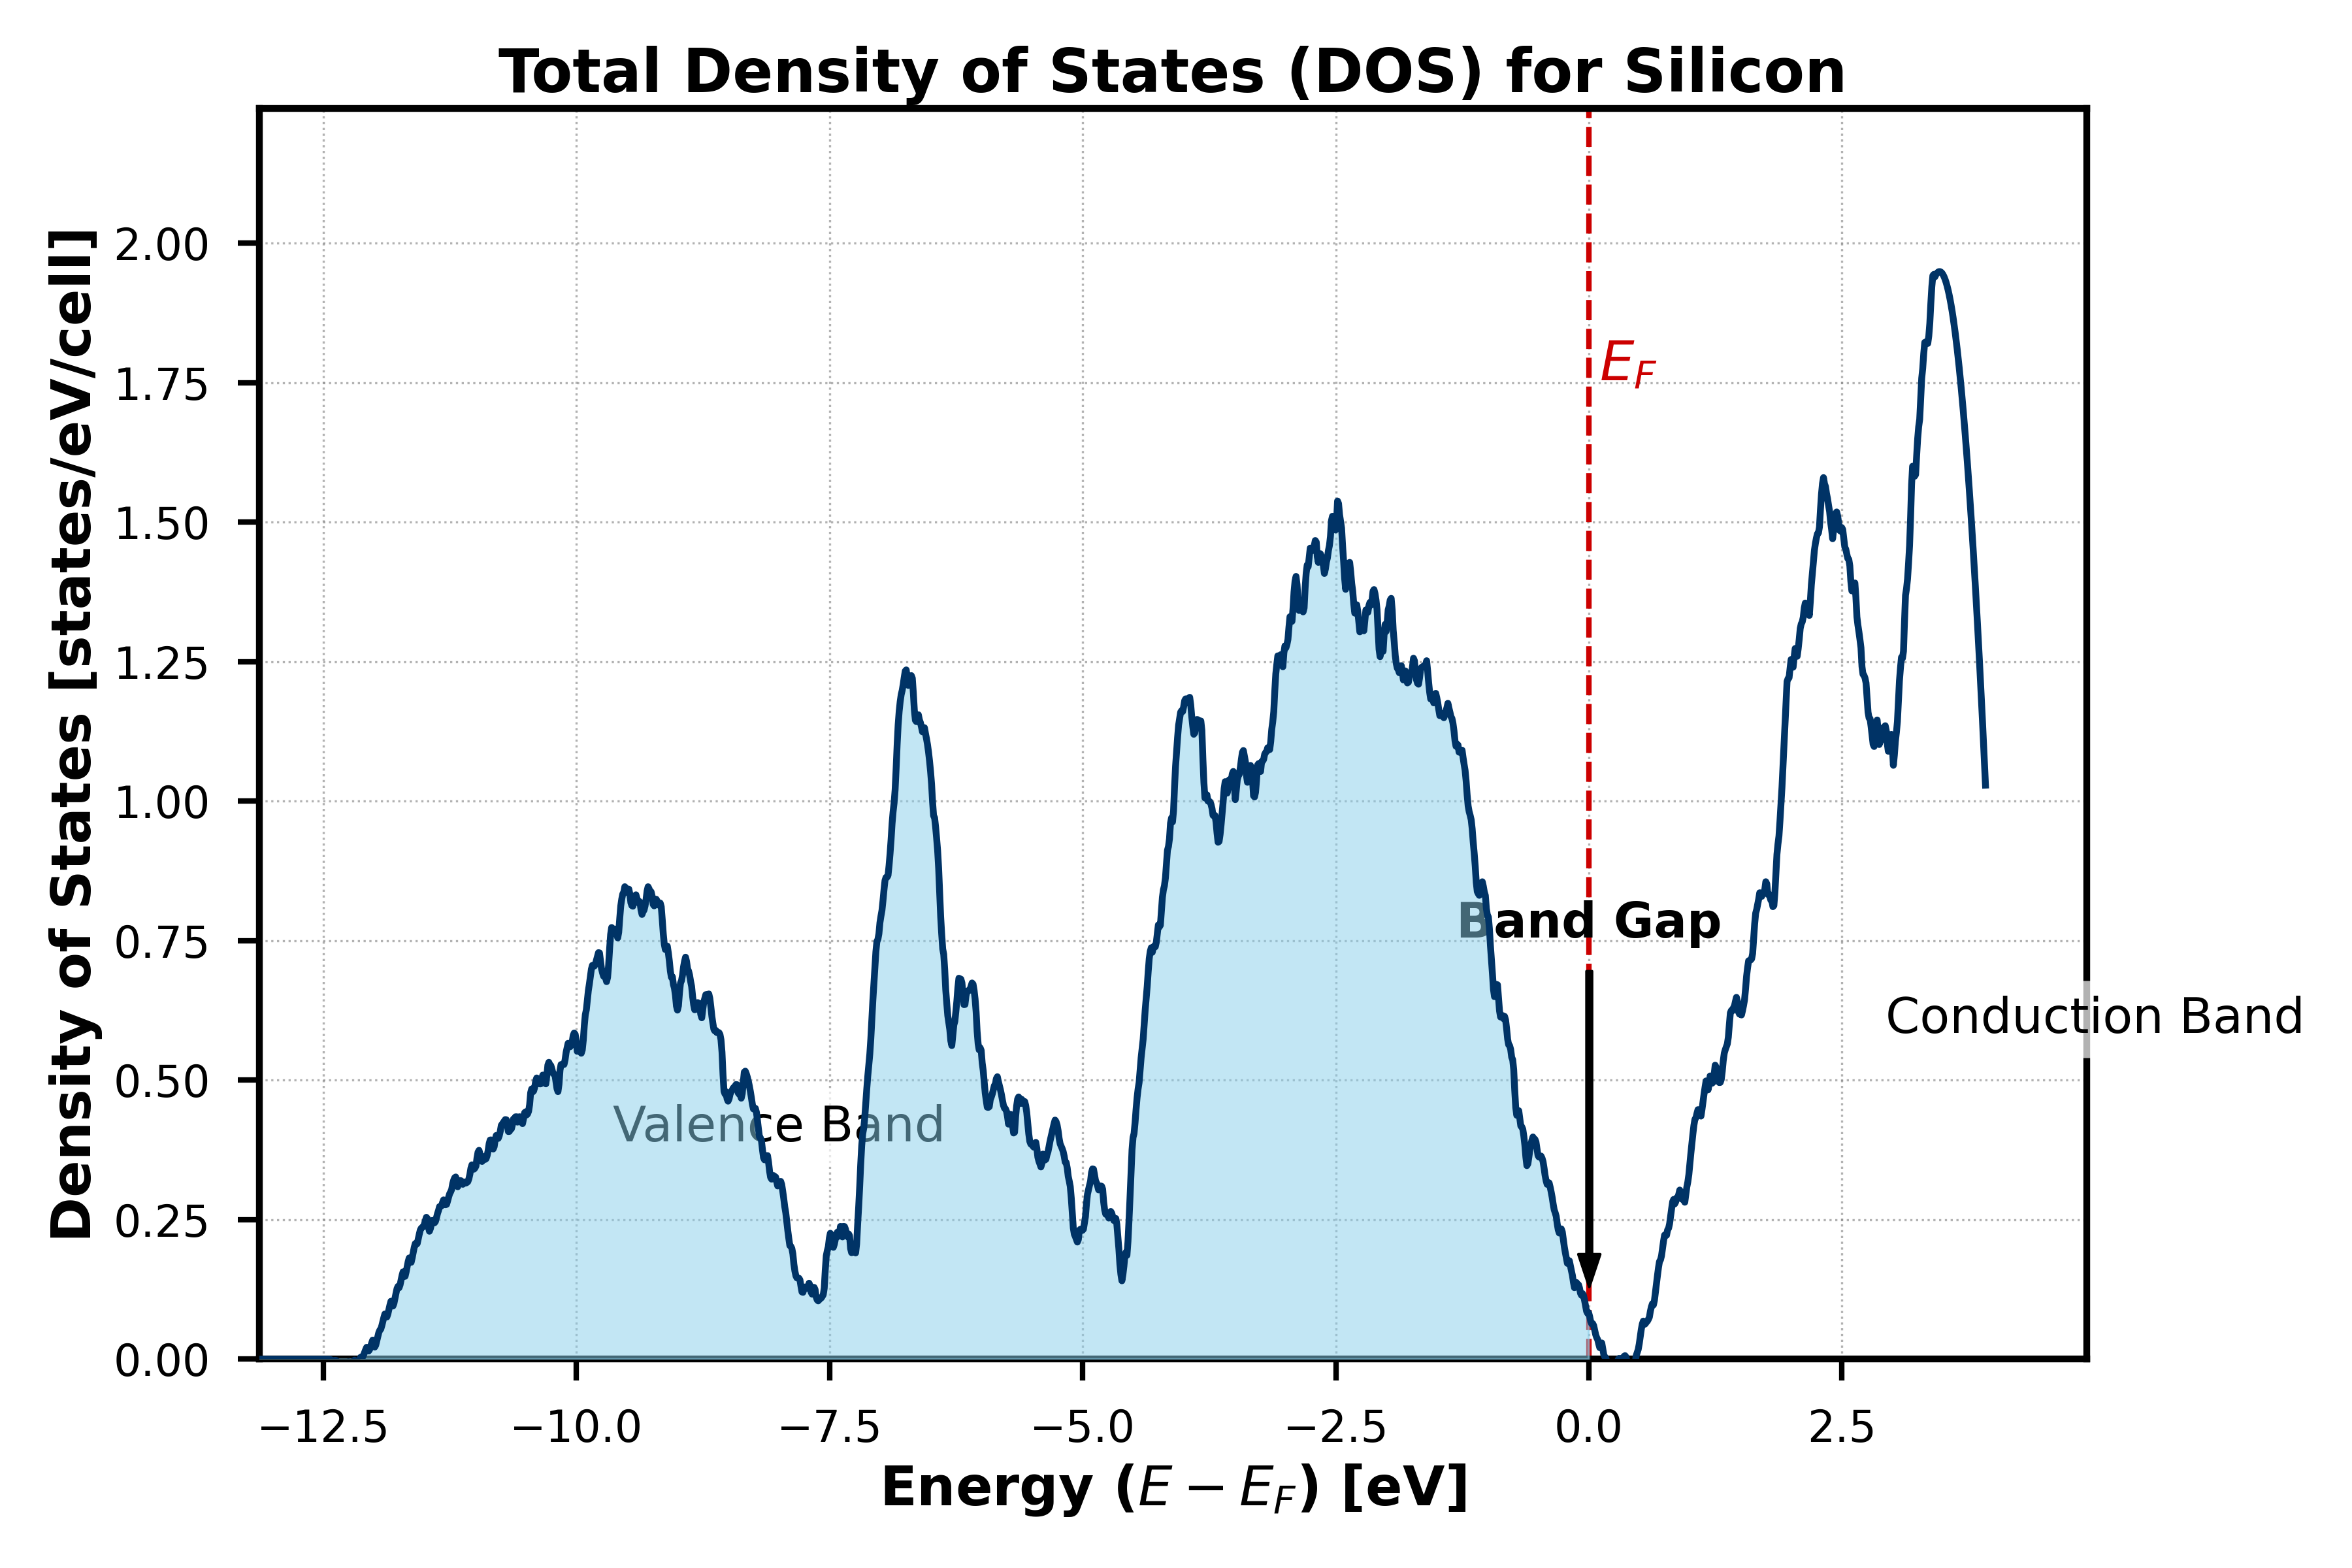
\includegraphics[width=0.7\textwidth]{img/silicon_dos_total_smooth_enhanced.png}
    \caption{Total Density of States (DOS) for silicon, calculated with DFT and smoothed using a Savitzky-Golay filter. The energy is referenced to the Fermi level ($E_F$), set at the Valence Band Maximum.}
    \label{fig:dos}
\end{figure}

The DOS of silicon in the diamond structure highlights features consistent with its semiconductor properties. In Fig. \ref{fig:dos}, we can observe three main regions:
\begin{itemize}
    \item \textbf{Valence band (E $< 0$ eV):} This region of occupied states extends down to approximately $-12.5\sim$ eV. It is characterized by a multi-peaked structure, which can be associated with the $sp^3$ hybridized orbitals typical of silicon's tetrahedral bonding. The prominent features include a peak corresponding to s-like states around $-10\sim$ eV and broader features from p-like states closer to the Fermi level.
    
    \item \textbf{Band gap:} A region of zero density of states is clearly visible around the Fermi level. The width of this gap, starting from $E-E_F = 0\sim$ eV, is approximately $1.0\sim$ eV. This value is in excellent agreement with the band gap of $1.010\sim$ eV determined from our previous band structure analysis. However, it shows the well-known underestimation typical of standard DFT approximations when compared to the experimental value of approximately $1.17\sim$ eV at low temperatures \cite{sze_2006, macfarlane_1958}. This discrepancy is primarily attributed to the self-interaction error inherent in many exchange-correlation functionals \cite{perdew_zunger_1981}.
    
    \item \textbf{Conduction band (E $> 1.0$ eV):} The DOS becomes non-zero again, indicating the availability of empty electronic states. This region shows a complex structure with distinct peaks, reflecting the intricate arrangement of the conduction bands.
\end{itemize}

In conclusion, the calculation of the density of states for silicon has yielded results that are in excellent agreement with both theoretical expectations and our own band structure calculations. The DOS plot clearly reveals the semiconductor nature of silicon with a band gap of approximately $1.0\sim$ eV. The structure of the valence and conduction bands accurately reflects the nature of covalent bonding in the silicon crystal. This analysis provides a comprehensive characterization of the electronic properties of crystalline silicon and validates our computational methodology.



\section{Phonon Frequency Calculation at the $\Gamma$-point}

In a periodic crystal lattice, the collective, quantized vibrations of atoms are described by quasiparticles known as phonons \cite{kittel_2005}. Phonons are fundamental to understanding many physical properties of solids, including thermal and electrical conductivity. Silicon, having a diamond lattice structure with two atoms in its primitive unit cell, exhibits both acoustic and optical phonon branches. At the zone center ($\Gamma$-point), the three acoustic modes have zero frequency, while the three optical modes are degenerate. The calculation of the frequency of these optical modes provides a stringent test for the accuracy of the interatomic forces predicted by our computational model.

To determine the frequency of the zone-center optical phonon, we employed a direct method based on \textit{ab initio} Molecular Dynamics (MD). This approach involves simulating the atomic motion in time and extracting the vibrational frequencies through a Fourier analysis of the atomic trajectory. The methodology was implemented as follows:

\begin{enumerate}
    \item \textbf{Excitation of the Optical Mode:} We first prepared the system to excite the desired vibrational mode. Starting from the optimized lattice structure, the two silicon atoms in the primitive cell were displaced from their equilibrium positions in opposite directions along the [$111$] crystallographic axis. This displacement breaks the symmetry and initiates an oscillation corresponding to the longitudinal/transverse optical (LO/TO) phonon at the $\Gamma$-point. The initial atomic positions were set to `Si $0.00$ $0.00$ $0.00$` and `Si $0.245$ $0.245$ $0.245$`.

    \item \textbf{Molecular Dynamics Simulation:} A microcanonical (NVE) MD simulation was performed using Quantum ESPRESSO. The system was allowed to evolve for $500$ time steps of $20\sim$ fs each, with the ionic equations of motion integrated using the Verlet algorithm. The forces on the atoms were calculated at each step using DFT, and the atomic positions were recorded to generate a trajectory.

    \item \textbf{Fourier Analysis:} The time series of the relative atomic displacement was then analyzed. After discarding the initial transient steps, we applied a Fast Fourier Transform (FFT) to the stable oscillatory motion to obtain its power spectrum. The dominant peak in the spectrum corresponds to the frequency of the excited phonon mode.
\end{enumerate}

Figure \ref{fig:phonon_oscillation} displays the relative displacement of the silicon atoms as a function of time, clearly showing the stable, periodic oscillation that serves as the input for our frequency analysis.

\begin{figure}[h!]
    \centering
    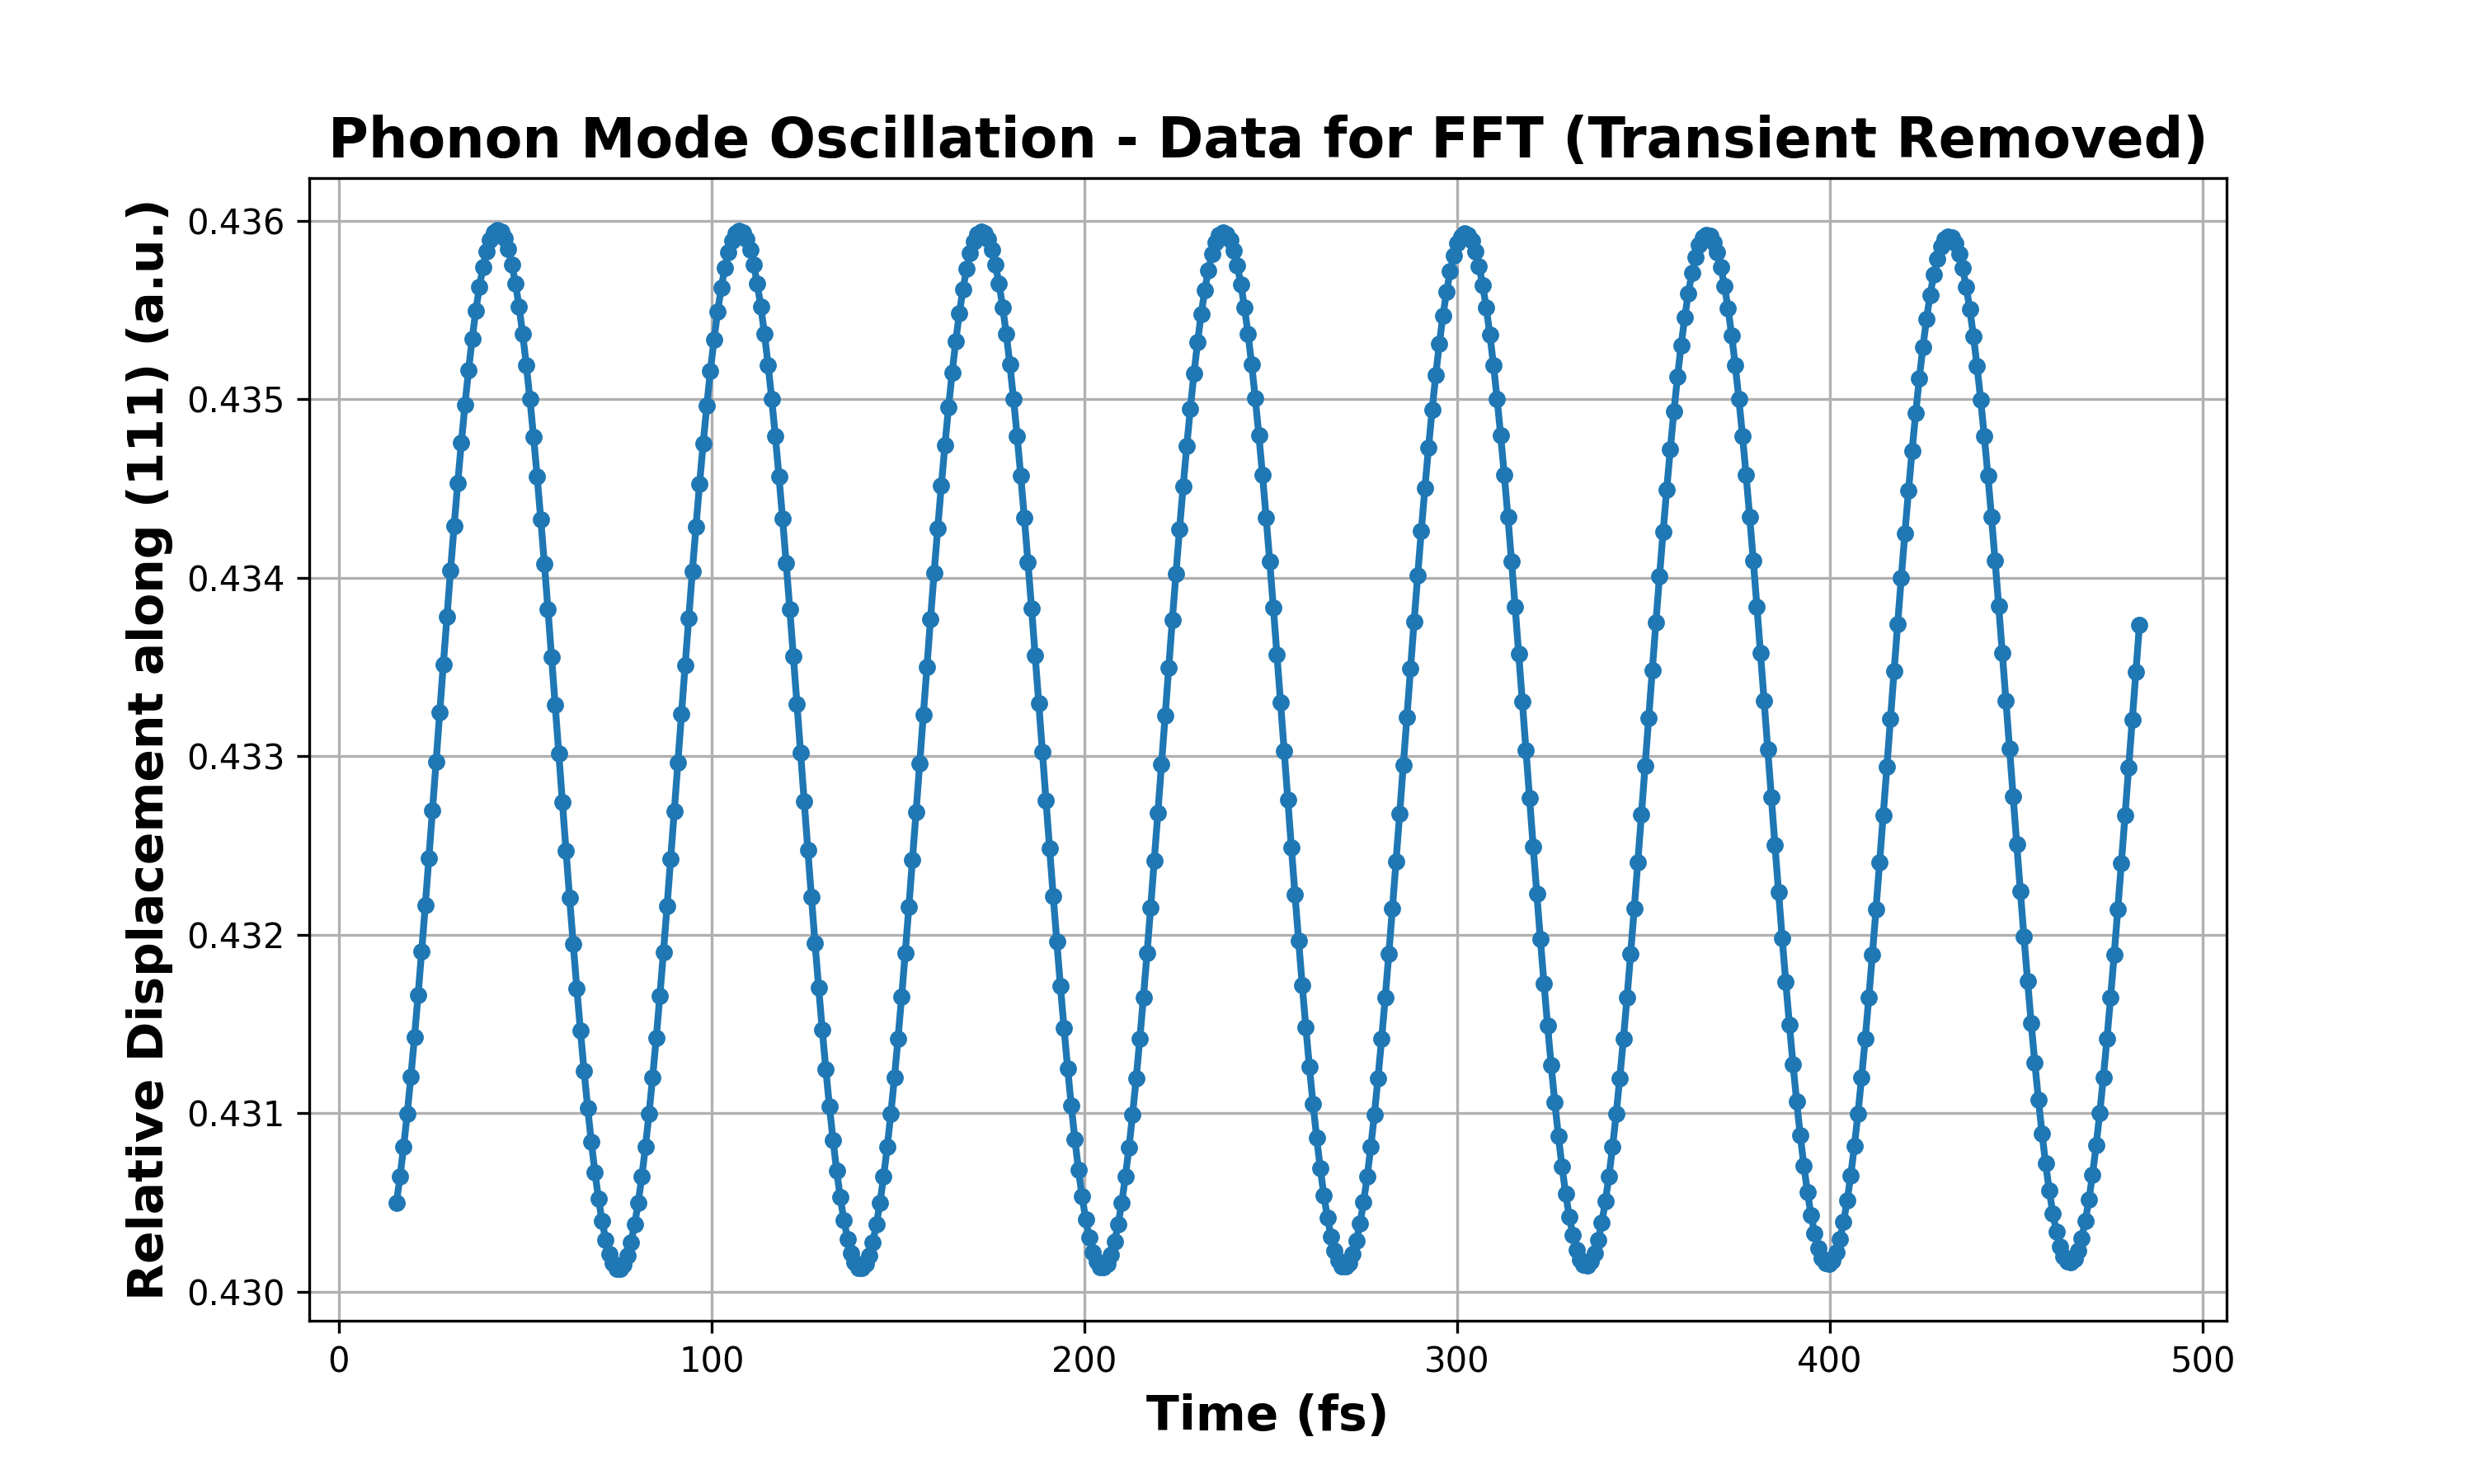
\includegraphics[width=0.7\textwidth]{img/displacement_time_clean.png} % NOME FILE MODIFICATO
    \caption{Time evolution of the relative atomic displacement of Si atoms along the [$111$] direction from the MD simulation. The data shows a stable oscillation after an initial transient period, characteristic of a phonon mode.}
    \label{fig:phonon_oscillation}
\end{figure}

The resulting Fourier spectrum is shown in Figure \ref{fig:phonon_fft}. A sharp and well-defined peak dominates the spectrum, unambiguously identifying the frequency of the zone-center optical phonon.

\begin{figure}[h!]
    \centering
    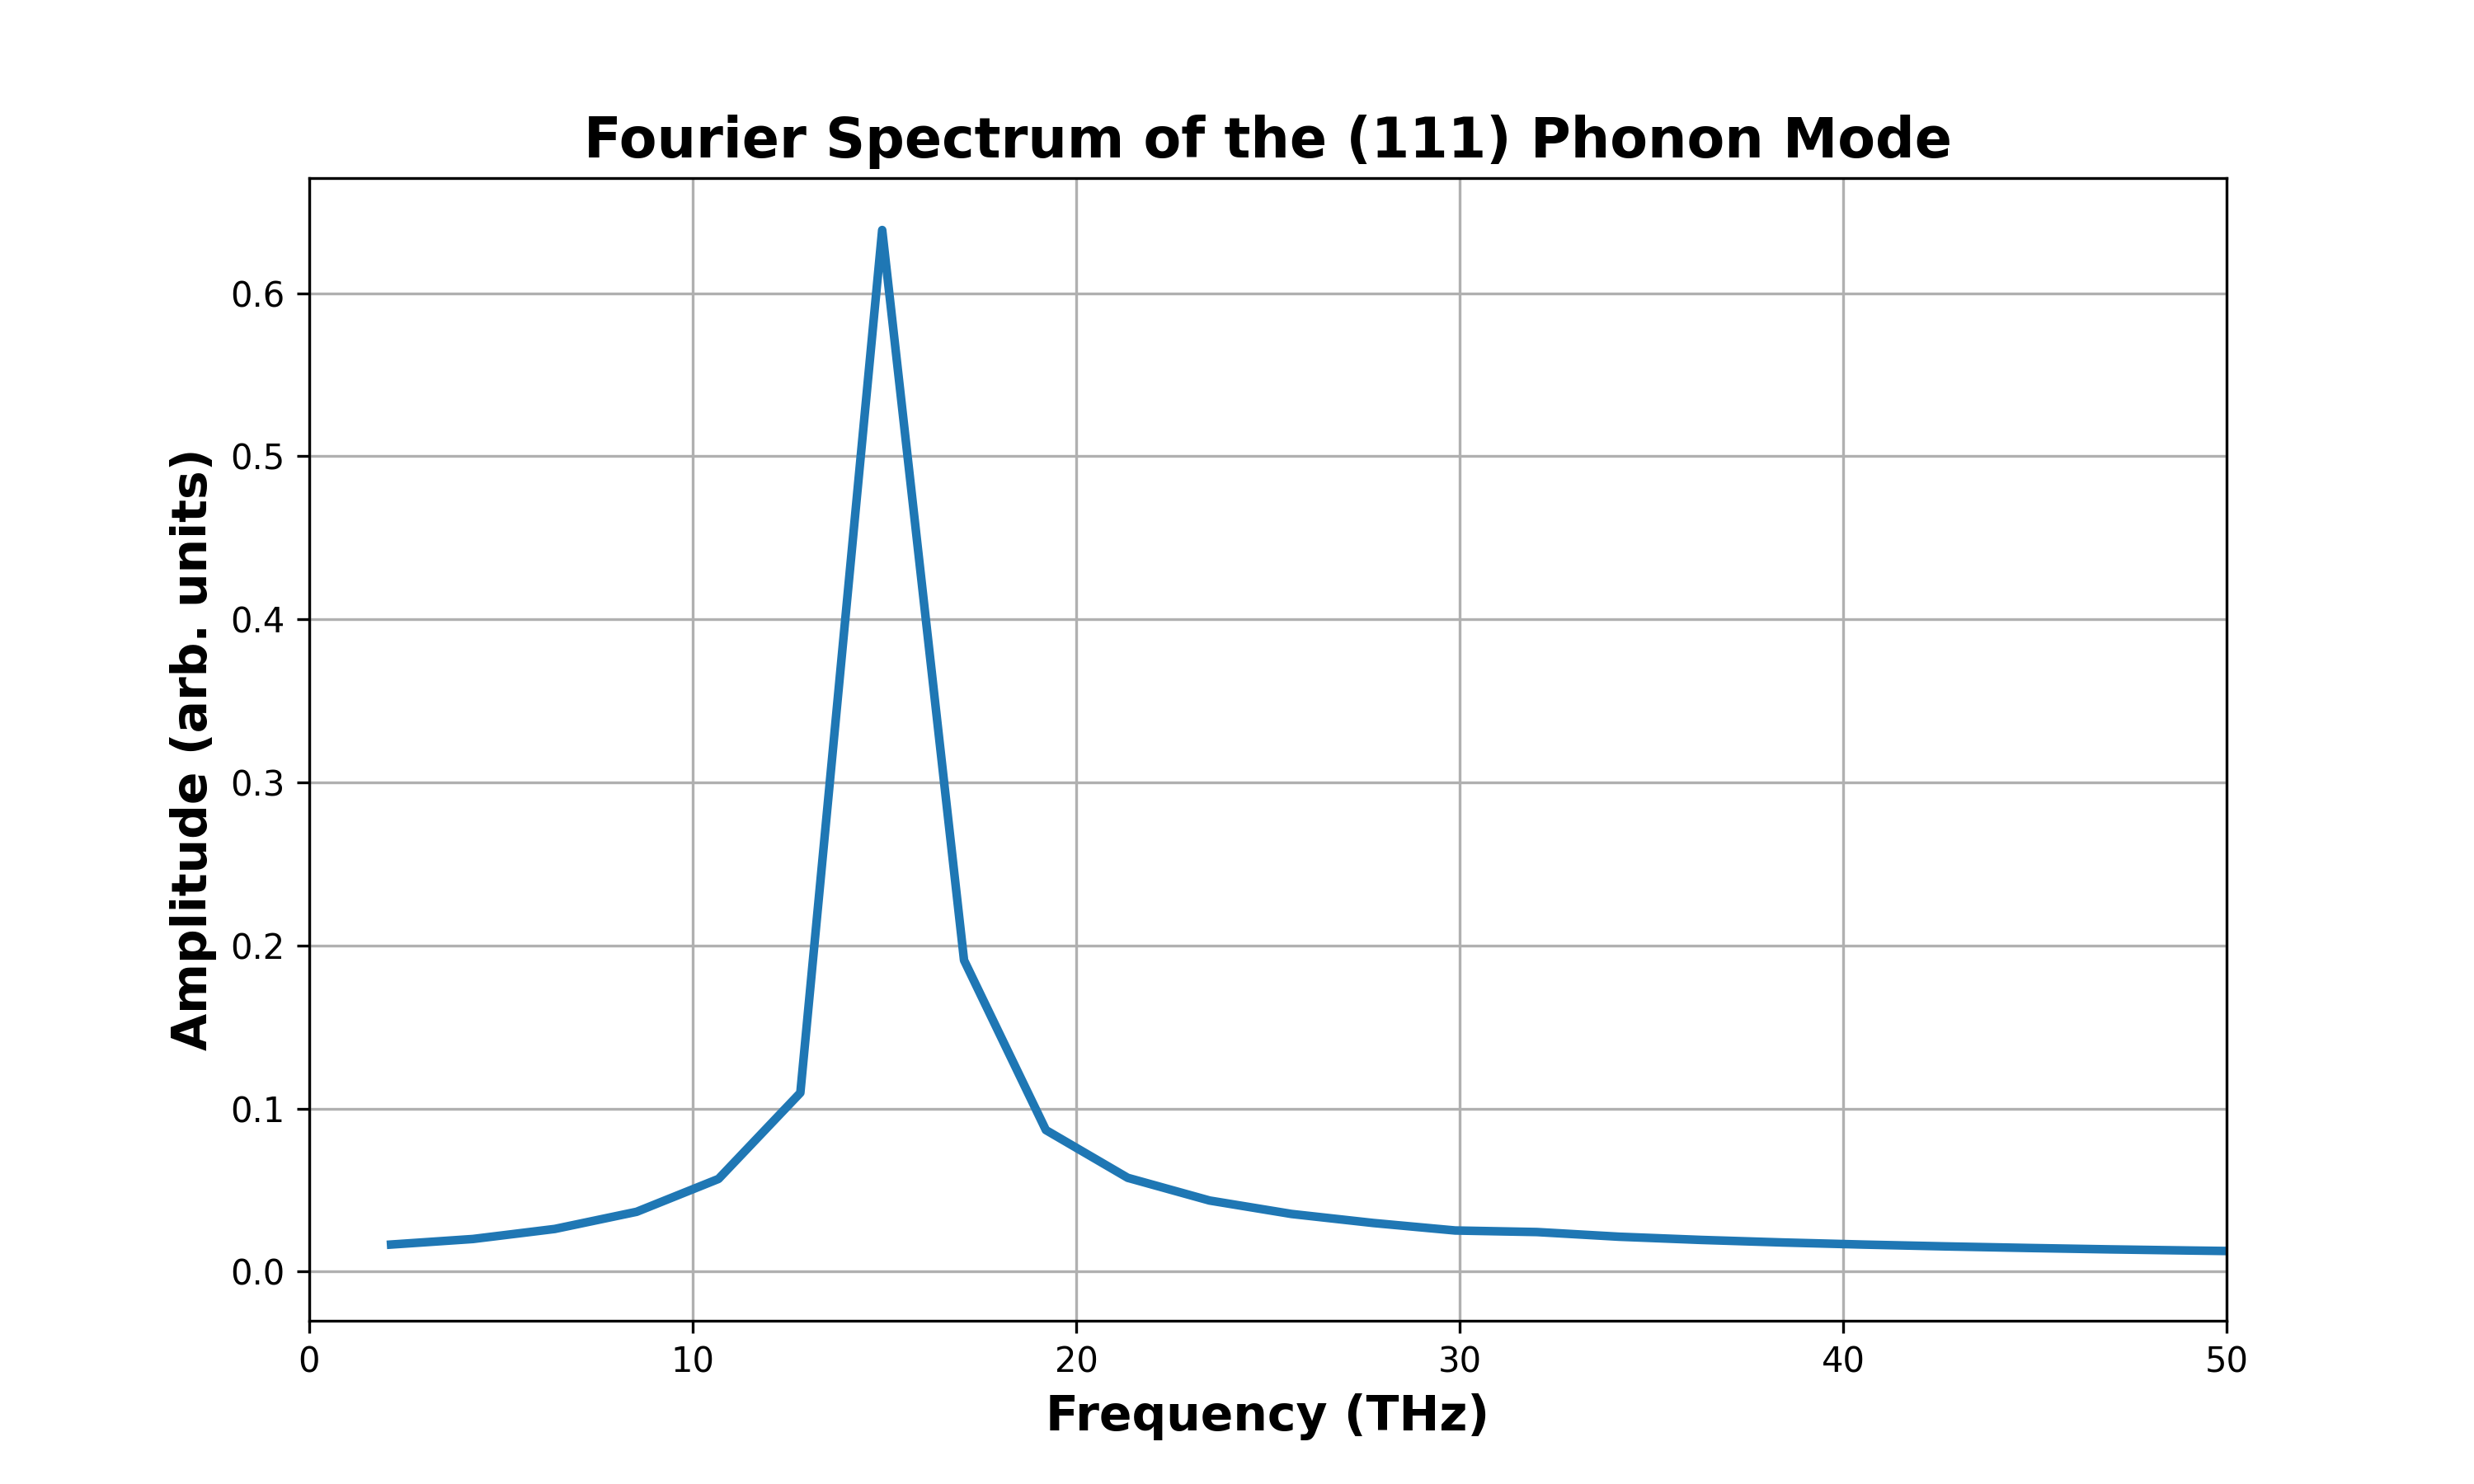
\includegraphics[width=0.7\textwidth]{img/frequency_spectrum.png} % NOME FILE MODIFICATO
    \caption{Fourier power spectrum of the atomic oscillation shown in Fig. \ref{fig:phonon_oscillation}. The dominant peak at $14.94\sim$ THz corresponds to the calculated frequency of the TO/LO phonon mode at the $\Gamma$-point.}
    \label{fig:phonon_fft}
\end{figure}

From the peak in the FFT spectrum, we determined the phonon frequency to be $14.94\sim$ THz. This result is compared with the well-established experimental value in Table \ref{tab:phonon_comparison}.

\begin{table}[h!]
    \centering
    \caption{Comparison of the calculated $\Gamma$-point optical phonon frequency with experimental data for silicon.}
    \label{tab:phonon_comparison} % Etichetta modificata per chiarezza
    \begin{tabular}{c c c}
        \hline\hline
         \textbf{Method} & \textbf{Frequency (THz)} & \textbf{Wavenumber (cm$^{-1}$)} \\
         \hline
         Experimental (LO/TO at $\Gamma$) & $15.52 \pm 0.15$ \cite{dolling_1963} & $517.7 \pm 5$ \cite{temple_1971} \\
         Our Calculation (MD + FFT) & $14.94$ & $498.3$ \\
         \hline\hline
    \end{tabular}
\end{table}

The calculated frequency of $14.94\sim$ THz shows excellent agreement with the experimental value of approximately $15.52\sim$ THz, with a relative deviation of only $3.7\%$. This small underestimation is a known feature of DFT calculations with standard exchange-correlation functionals (like PBE), which tend to slightly underestimate the bond stiffness and, consequently, the vibrational frequencies. The high accuracy of our result validates the quality of the interatomic forces predicted by our DFT model and demonstrates the reliability of the MD-based approach for calculating vibrational properties.


\section{Conclusion}

In this work, we have performed a comprehensive computational characterization of the fundamental structural, electronic, and vibrational properties of crystalline silicon using Density Functional Theory. By systematically applying a well-defined and converged methodology, we have obtained results that are in excellent quantitative and qualitative agreement with decades of experimental research.

Our analysis began with the determination of the equilibrium lattice constant ($a_0 = 5.416\sim$ \AA) and bulk modulus ($B_0 = 93.3\sim$ GPa), which were found to be in excellent agreement with experimental measurements, exhibiting the slight underestimation characteristic of the PBE functional.

The investigation of the electronic properties successfully reproduced the indirect nature of silicon's band gap, with a calculated value of $1.010\sim$ eV. This result, corroborated by the Density of States analysis, aligns with the known tendency of semi-local functionals to underestimate the experimental gap, while correctly describing the overall band topology and key features of the electronic structure.

Furthermore, the calculation of the zone-center optical phonon frequency ($14.94\sim$ THz) via \textit{ab initio} molecular dynamics yielded a value remarkably close to experimental data, validating the accuracy of the interatomic forces predicted by our model.

Taken together, these results demonstrate a consistent and robust picture. The PBE functional, despite its known limitations, proves to be a reliable and highly effective tool for predicting a wide range of physical properties of silicon with high accuracy. This work not only reinforces our understanding of silicon but also serves as a validation of the computational methodology, highlighting its power as a predictive and insightful tool in modern materials science.

\printbibliography %Prints bibliography
%1 2 3 4 5 6 7 8 9 10 11 12 vì
\end{document}
